% !TeX program = xelatex
\documentclass[12pt, a4paper]{article}
\usepackage{amsmath}
\usepackage{xeCJK}
\usepackage{amsmath}
\usepackage{amssymb}
\usepackage{xcolor}
\usepackage{parskip}
\usepackage{tikz}
\usepackage{enumitem}

\setmainfont{Latin Modern Roman}
\setCJKmainfont{Noto Serif CJK TC}

\title{BJT}

\begin{document}
\section*{Concept of BJT}
\begin{center}
	

\tikzset{every picture/.style={line width=0.75pt}} %set default line width to 0.75pt        

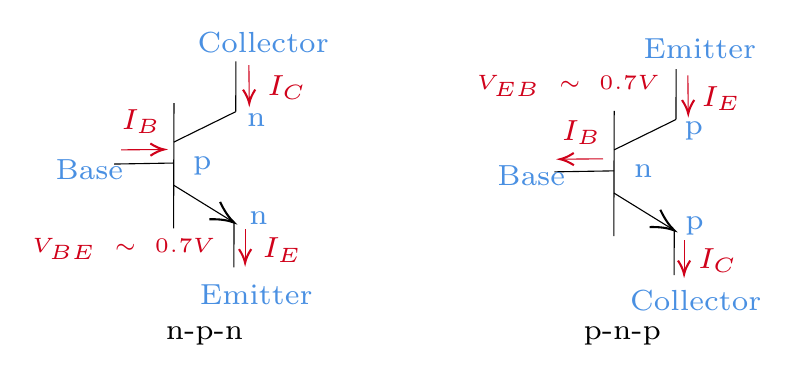
\begin{tikzpicture}[x=0.75pt,y=0.75pt,yscale=-1,xscale=1]
%uncomment if require: \path (0,300); %set diagram left start at 0, and has height of 300

%Straight Lines [id:da41720361884938184] 
\draw    (456.19,110.91) -- (456.13,129.72) -- (456.1,139.82) -- (456.07,150.51) -- (456,171.26) ;
%Straight Lines [id:da6884450440198249] 
\draw    (456.13,129.72) -- (485.95,115.07) ;
%Straight Lines [id:da4299314098075526] 
\draw    (456.07,150.51) -- (483.43,167.42) ;
\draw [shift={(485.13,168.47)}, rotate = 211.73] [color={rgb, 255:red, 0; green, 0; blue, 0 }  ][line width=0.75]    (10.93,-4.9) .. controls (6.95,-2.3) and (3.31,-0.67) .. (0,0) .. controls (3.31,0.67) and (6.95,2.3) .. (10.93,4.9)   ;
%Straight Lines [id:da99953250770795] 
\draw    (485.95,115.07) -- (486.03,90.84) ;
%Straight Lines [id:da16894446125496687] 
\draw    (485.13,168.47) -- (485.03,190.07) ;
%Straight Lines [id:da27628282565223083] 
\draw    (427.38,140.3) -- (456.1,139.82) ;
%Straight Lines [id:da5756441571661479] 
\draw    (244.09,107.15) -- (244.03,125.96) -- (244,136.05) -- (243.97,146.74) -- (243.9,167.49) ;
%Straight Lines [id:da06709557802156885] 
\draw    (244.03,125.96) -- (273.85,111.3) ;
%Straight Lines [id:da5280630440607302] 
\draw    (243.97,146.74) -- (271.33,163.66) ;
\draw [shift={(273.03,164.71)}, rotate = 211.73] [color={rgb, 255:red, 0; green, 0; blue, 0 }  ][line width=0.75]    (10.93,-4.9) .. controls (6.95,-2.3) and (3.31,-0.67) .. (0,0) .. controls (3.31,0.67) and (6.95,2.3) .. (10.93,4.9)   ;
%Straight Lines [id:da836552250786984] 
\draw    (273.85,111.3) -- (273.93,87.07) ;
%Straight Lines [id:da30921103922378723] 
\draw    (273.03,164.71) -- (272.93,186.3) ;
%Straight Lines [id:da18564800925517488] 
\draw    (215.28,136.54) -- (244,136.05) ;
%Straight Lines [id:da26678801997549273] 
\draw [color={rgb, 255:red, 208; green, 2; blue, 27 }  ,draw opacity=1 ]   (432.16,134.18) -- (450.79,134.02) ;
\draw [shift={(430.16,134.2)}, rotate = 359.51] [color={rgb, 255:red, 208; green, 2; blue, 27 }  ,draw opacity=1 ][line width=0.75]    (6.56,-2.94) .. controls (4.17,-1.38) and (1.99,-0.4) .. (0,0) .. controls (1.99,0.4) and (4.17,1.38) .. (6.56,2.94)   ;
%Straight Lines [id:da8448156798036344] 
\draw [color={rgb, 255:red, 208; green, 2; blue, 27 }  ,draw opacity=1 ]   (491.84,110.24) -- (491.68,93.87) ;
\draw [shift={(491.86,112.24)}, rotate = 269.46] [color={rgb, 255:red, 208; green, 2; blue, 27 }  ,draw opacity=1 ][line width=0.75]    (6.56,-2.94) .. controls (4.17,-1.38) and (1.99,-0.4) .. (0,0) .. controls (1.99,0.4) and (4.17,1.38) .. (6.56,2.94)   ;
%Straight Lines [id:da45090343003545064] 
\draw [color={rgb, 255:red, 208; green, 2; blue, 27 }  ,draw opacity=1 ]   (489.86,187.6) -- (489.86,173.31) ;
\draw [shift={(489.86,189.6)}, rotate = 270] [color={rgb, 255:red, 208; green, 2; blue, 27 }  ,draw opacity=1 ][line width=0.75]    (6.56,-2.94) .. controls (4.17,-1.38) and (1.99,-0.4) .. (0,0) .. controls (1.99,0.4) and (4.17,1.38) .. (6.56,2.94)   ;
%Straight Lines [id:da08583927969420024] 
\draw [color={rgb, 255:red, 208; green, 2; blue, 27 }  ,draw opacity=1 ]   (280.34,105.24) -- (280.18,88.87) ;
\draw [shift={(280.36,107.24)}, rotate = 269.46] [color={rgb, 255:red, 208; green, 2; blue, 27 }  ,draw opacity=1 ][line width=0.75]    (6.56,-2.94) .. controls (4.17,-1.38) and (1.99,-0.4) .. (0,0) .. controls (1.99,0.4) and (4.17,1.38) .. (6.56,2.94)   ;
%Straight Lines [id:da23637271134315985] 
\draw [color={rgb, 255:red, 208; green, 2; blue, 27 }  ,draw opacity=1 ]   (278.36,182.1) -- (278.36,167.81) ;
\draw [shift={(278.36,184.1)}, rotate = 270] [color={rgb, 255:red, 208; green, 2; blue, 27 }  ,draw opacity=1 ][line width=0.75]    (6.56,-2.94) .. controls (4.17,-1.38) and (1.99,-0.4) .. (0,0) .. controls (1.99,0.4) and (4.17,1.38) .. (6.56,2.94)   ;
%Straight Lines [id:da4645166143519025] 
\draw [color={rgb, 255:red, 208; green, 2; blue, 27 }  ,draw opacity=1 ]   (218.66,129.7) -- (237.29,129.54) ;
\draw [shift={(239.29,129.52)}, rotate = 179.51] [color={rgb, 255:red, 208; green, 2; blue, 27 }  ,draw opacity=1 ][line width=0.75]    (6.56,-2.94) .. controls (4.17,-1.38) and (1.99,-0.4) .. (0,0) .. controls (1.99,0.4) and (4.17,1.38) .. (6.56,2.94)   ;

% Text Node
\draw (253.62,71.1) node [anchor=north west][inner sep=0.75pt]  [font=\scriptsize,color={rgb, 255:red, 74; green, 144; blue, 226 }  ,opacity=1 ,xscale=1.5,yscale=1.5] [align=left] {Collector};
% Text Node
\draw (462.02,195.57) node [anchor=north west][inner sep=0.75pt]  [font=\scriptsize,color={rgb, 255:red, 74; green, 144; blue, 226 }  ,opacity=1 ,xscale=1.5,yscale=1.5] [align=left] {Collector};
% Text Node
\draw (254.72,192.8) node [anchor=north west][inner sep=0.75pt]  [font=\scriptsize,color={rgb, 255:red, 74; green, 144; blue, 226 }  ,opacity=1 ,xscale=1.5,yscale=1.5] [align=left] {Emitter};
% Text Node
\draw (468.42,74.14) node [anchor=north west][inner sep=0.75pt]  [font=\scriptsize,color={rgb, 255:red, 74; green, 144; blue, 226 }  ,opacity=1 ,xscale=1.5,yscale=1.5] [align=left] {Emitter};
% Text Node
\draw (398.02,135.17) node [anchor=north west][inner sep=0.75pt]  [font=\scriptsize,color={rgb, 255:red, 74; green, 144; blue, 226 }  ,opacity=1 ,xscale=1.5,yscale=1.5] [align=left] {Base};
% Text Node
\draw (185.12,132.37) node [anchor=north west][inner sep=0.75pt]  [font=\scriptsize,color={rgb, 255:red, 74; green, 144; blue, 226 }  ,opacity=1 ,xscale=1.5,yscale=1.5] [align=left] {Base};
% Text Node
\draw (463.91,135.17) node [anchor=north west][inner sep=0.75pt]  [font=\scriptsize,color={rgb, 255:red, 74; green, 144; blue, 226 }  ,opacity=1 ,xscale=1.5,yscale=1.5] [align=left] {n};
% Text Node
\draw (277.41,110.33) node [anchor=north west][inner sep=0.75pt]  [font=\scriptsize,color={rgb, 255:red, 74; green, 144; blue, 226 }  ,opacity=1 ,xscale=1.5,yscale=1.5] [align=left] {n};
% Text Node
\draw (278.57,157.83) node [anchor=north west][inner sep=0.75pt]  [font=\scriptsize,color={rgb, 255:red, 74; green, 144; blue, 226 }  ,opacity=1 ,xscale=1.5,yscale=1.5] [align=left] {n};
% Text Node
\draw (488.19,114.4) node [anchor=north west][inner sep=0.75pt]  [font=\scriptsize,color={rgb, 255:red, 74; green, 144; blue, 226 }  ,opacity=1 ,xscale=1.5,yscale=1.5] [align=left] {p};
% Text Node
\draw (488.57,160.12) node [anchor=north west][inner sep=0.75pt]  [font=\scriptsize,color={rgb, 255:red, 74; green, 144; blue, 226 }  ,opacity=1 ,xscale=1.5,yscale=1.5] [align=left] {p};
% Text Node
\draw (251.41,131) node [anchor=north west][inner sep=0.75pt]  [font=\scriptsize,color={rgb, 255:red, 74; green, 144; blue, 226 }  ,opacity=1 ,xscale=1.5,yscale=1.5] [align=left] {p};
% Text Node
\draw (439.57,213.33) node [anchor=north west][inner sep=0.75pt]  [font=\scriptsize,xscale=1.5,yscale=1.5] [align=left] {p-n-p};
% Text Node
\draw (238.24,213.17) node [anchor=north west][inner sep=0.75pt]  [font=\scriptsize,xscale=1.5,yscale=1.5] [align=left] {n-p-n};
% Text Node
\draw (429.21,113.85) node [anchor=north west][inner sep=0.75pt]  [font=\scriptsize,color={rgb, 255:red, 208; green, 2; blue, 27 }  ,opacity=1 ,xscale=1.5,yscale=1.5]  {$I_{B}$};
% Text Node
\draw (496.54,97.27) node [anchor=north west][inner sep=0.75pt]  [font=\scriptsize,color={rgb, 255:red, 208; green, 2; blue, 27 }  ,opacity=1 ,xscale=1.5,yscale=1.5]  {$I_{E}$};
% Text Node
\draw (494.83,175.51) node [anchor=north west][inner sep=0.75pt]  [font=\scriptsize,color={rgb, 255:red, 208; green, 2; blue, 27 }  ,opacity=1 ,xscale=1.5,yscale=1.5]  {$I_{C}$};
% Text Node
\draw (388.03,91.81) node [anchor=north west][inner sep=0.75pt]  [font=\tiny,color={rgb, 255:red, 208; green, 2; blue, 27 }  ,opacity=1 ,xscale=1.5,yscale=1.5]  {$V_{EB} \ \sim \ 0.7V$};
% Text Node
\draw (285.04,170.27) node [anchor=north west][inner sep=0.75pt]  [font=\scriptsize,color={rgb, 255:red, 208; green, 2; blue, 27 }  ,opacity=1 ,xscale=1.5,yscale=1.5]  {$I_{E}$};
% Text Node
\draw (287.33,92.01) node [anchor=north west][inner sep=0.75pt]  [font=\scriptsize,color={rgb, 255:red, 208; green, 2; blue, 27 }  ,opacity=1 ,xscale=1.5,yscale=1.5]  {$I_{C}$};
% Text Node
\draw (217.04,108.35) node [anchor=north west][inner sep=0.75pt]  [font=\scriptsize,color={rgb, 255:red, 208; green, 2; blue, 27 }  ,opacity=1 ,xscale=1.5,yscale=1.5]  {$I_{B}$};
% Text Node
\draw (173.87,170.31) node [anchor=north west][inner sep=0.75pt]  [font=\tiny,color={rgb, 255:red, 208; green, 2; blue, 27 }  ,opacity=1 ,xscale=1.5,yscale=1.5]  {$V_{BE} \ \sim \ 0.7V$};
\end{tikzpicture}
\end{center}

\subsection*{Active mode}
B-E junction: \textbf{Forward bias} $\sim 0.7$V in general \\
B-C junction: \textbf{Reverse bias} or forward bias $<0.4$V

\subsection*{Saturation mode}
B-E junction: forward bias\\
B-C junction: forward bias \textcolor{red}> \textcolor{black}0.4V

\subsection*{Reverse active(Cut-off)}
B-E junction: reverse bias\\
B-C junction: forward bias
\newpage

\section*{Equation of BJT}

\begin{center}
\tikzset{every picture/.style={line width=0.75pt}} %set default line width to 0.75pt        

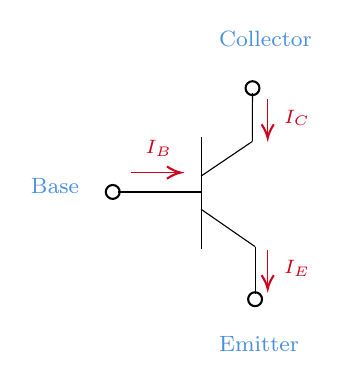
\begin{tikzpicture}[x=0.75pt,y=0.75pt,yscale=-1,xscale=1]
%uncomment if require: \path (0,300); %set diagram left start at 0, and has height of 300

%Straight Lines [id:da21757148579979202] 
\draw    (270.52,94.89) -- (270.52,113.56) -- (270.52,121.21) -- (270.52,129.56) -- (270.52,148.89) ;
%Straight Lines [id:da25534728237338333] 
\draw    (270.52,113.56) -- (295.18,96.89) ;
%Straight Lines [id:da07586494603654681] 
\draw    (270.52,129.56) -- (296.52,147.56) ;
%Straight Lines [id:da7075217700722117] 
\draw    (296.52,147.56) -- (296.52,170.54) ;
\draw [shift={(296.52,172.89)}, rotate = 90] [color={rgb, 255:red, 0; green, 0; blue, 0 }  ][line width=0.75]      (0, 0) circle [x radius= 3.35, y radius= 3.35]   ;
%Straight Lines [id:da7681202035592422] 
\draw    (295.26,73.56) -- (295.18,96.89) ;
\draw [shift={(295.27,71.21)}, rotate = 90.19] [color={rgb, 255:red, 0; green, 0; blue, 0 }  ][line width=0.75]      (0, 0) circle [x radius= 3.35, y radius= 3.35]   ;
%Straight Lines [id:da06169247997439231] 
\draw    (230.29,121.21) -- (270.52,121.21) ;
\draw [shift={(227.94,121.21)}, rotate = 0] [color={rgb, 255:red, 0; green, 0; blue, 0 }  ][line width=0.75]      (0, 0) circle [x radius= 3.35, y radius= 3.35]   ;
%Straight Lines [id:da6741645038870837] 
\draw [color={rgb, 255:red, 208; green, 2; blue, 27 }  ,draw opacity=1 ]   (236.6,111.88) -- (258.6,111.88) ;
\draw [shift={(260.6,111.88)}, rotate = 180] [color={rgb, 255:red, 208; green, 2; blue, 27 }  ,draw opacity=1 ][line width=0.75]    (6.56,-2.94) .. controls (4.17,-1.38) and (1.99,-0.4) .. (0,0) .. controls (1.99,0.4) and (4.17,1.38) .. (6.56,2.94)   ;
%Straight Lines [id:da794298671098817] 
\draw [color={rgb, 255:red, 208; green, 2; blue, 27 }  ,draw opacity=1 ]   (302.6,76.54) -- (302.6,93.21) ;
\draw [shift={(302.6,95.21)}, rotate = 270] [color={rgb, 255:red, 208; green, 2; blue, 27 }  ,draw opacity=1 ][line width=0.75]    (6.56,-2.94) .. controls (4.17,-1.38) and (1.99,-0.4) .. (0,0) .. controls (1.99,0.4) and (4.17,1.38) .. (6.56,2.94)   ;
%Straight Lines [id:da8468813132864502] 
\draw [color={rgb, 255:red, 208; green, 2; blue, 27 }  ,draw opacity=1 ]   (302.6,149.21) -- (302.6,165.88) ;
\draw [shift={(302.6,167.88)}, rotate = 270] [color={rgb, 255:red, 208; green, 2; blue, 27 }  ,draw opacity=1 ][line width=0.75]    (6.56,-2.94) .. controls (4.17,-1.38) and (1.99,-0.4) .. (0,0) .. controls (1.99,0.4) and (4.17,1.38) .. (6.56,2.94)   ;

% Text Node
\draw (242.55,95.07) node [anchor=north west][inner sep=0.75pt]  [font=\scriptsize,color={rgb, 255:red, 208; green, 2; blue, 27 }  ,opacity=1 ]  {$I_{B}$};
% Text Node
\draw (309.22,80.4) node [anchor=north west][inner sep=0.75pt]  [font=\scriptsize,color={rgb, 255:red, 208; green, 2; blue, 27 }  ,opacity=1 ]  {$I_{C}$};
% Text Node
\draw (309.22,153.07) node [anchor=north west][inner sep=0.75pt]  [font=\scriptsize,color={rgb, 255:red, 208; green, 2; blue, 27 }  ,opacity=1 ]  {$I_{E}$};
% Text Node
\draw (277.88,42.33) node [anchor=north west][inner sep=0.75pt]  [font=\footnotesize,color={rgb, 255:red, 74; green, 144; blue, 226 }  ,opacity=1 ] [align=left] {Collector};
% Text Node
\draw (277.88,189.67) node [anchor=north west][inner sep=0.75pt]  [font=\footnotesize,color={rgb, 255:red, 74; green, 144; blue, 226 }  ,opacity=1 ] [align=left] {Emitter};
% Text Node
\draw (187.22,113.33) node [anchor=north west][inner sep=0.75pt]  [font=\footnotesize,color={rgb, 255:red, 74; green, 144; blue, 226 }  ,opacity=1 ] [align=left] {Base};
\end{tikzpicture}
\end{center}

$i_C$ 有三種表示法
\begin{align*}
	i_C &= I_s \exp(\frac{V_{BE}}{V_T}) \\
	i_C &= \alpha i_E \\
	i_C &= \beta i_B
\end{align*}
By KCL, we have
\begin{align*}
	i_E &= i_C + i_B = (1 + \beta) i_B \\
	\alpha &= \frac{\beta}{1 + \beta}
\end{align*}

\subsection*{Activate Mode}
在Activate region 可以直接用$V_{BE} \sim 0.7$V 進行解題。 \\
算完後要確認 $V_{CE} > 0.3$V,如果沒有則為 Saturatino mode,要用 Saturation 再解一次 

\subsection*{Saturation Mode}
可以直接將 $V_{CE}$ 假設成 0.2V \\
$V_{BE}$ 一樣是用 0.7V 計算

\newpage


\section*{Early effect}
$V_{CE}$ 增加 $\to V_{CB}$ 增加 $\to$ B-C 空乏區增加 $\to$ Base 的寬度下降 $\to$ 濃度斜率 $\frac{\text{d}n_p(x)}{\text{d}x}$ 會增加 $\to$ 擴散下降 $\to i_C$ 上升 

\begin{center}


\tikzset{every picture/.style={line width=0.75pt}} %set default line width to 0.75pt        

\begin{tikzpicture}[x=0.75pt,y=0.75pt,yscale=-1,xscale=1]
%uncomment if require: \path (0,300); %set diagram left start at 0, and has height of 300

%Shape: Axis 2D [id:dp7006808894110714] 
\draw  (89.4,197.95) -- (476.9,197.95)(329.9,57) -- (329.9,233.5) (469.9,192.95) -- (476.9,197.95) -- (469.9,202.95) (324.9,64) -- (329.9,57) -- (334.9,64)  ;
%Curve Lines [id:da1662617910736548] 
\draw [color={rgb, 255:red, 74; green, 144; blue, 226 }  ,draw opacity=1 ] [dash pattern={on 0.84pt off 2.51pt}]  (329.9,199.5) .. controls (335.4,144.95) and (324.4,127.45) .. (428.4,130.45) ;
%Curve Lines [id:da4110110332494028] 
\draw [color={rgb, 255:red, 74; green, 144; blue, 226 }  ,draw opacity=1 ] [dash pattern={on 0.84pt off 2.51pt}]  (329.9,199.5) .. controls (331.9,176.95) and (361.9,181.95) .. (427.9,181.45) ;
%Curve Lines [id:da4269246396008519] 
\draw [color={rgb, 255:red, 74; green, 144; blue, 226 }  ,draw opacity=1 ] [dash pattern={on 0.84pt off 2.51pt}]  (329.9,199.5) .. controls (332.9,150.45) and (355.9,161.45) .. (428.9,159.95) ;
%Curve Lines [id:da3515975411569565] 
\draw [color={rgb, 255:red, 245; green, 166; blue, 35 }  ,draw opacity=1 ]   (329.9,199.5) .. controls (331.9,133.45) and (330.9,140.95) .. (424.4,118.45) ;
%Curve Lines [id:da5183570912397766] 
\draw [color={rgb, 255:red, 245; green, 166; blue, 35 }  ,draw opacity=1 ]   (329.9,199.5) .. controls (325.4,158.45) and (354.9,161.45) .. (425.4,150.45) ;
%Curve Lines [id:da7123319531540379] 
\draw [color={rgb, 255:red, 245; green, 166; blue, 35 }  ,draw opacity=1 ]   (329.9,199.5) .. controls (328.4,182.45) and (355.9,173.25) .. (425.4,170.45) ;
%Straight Lines [id:da22054102568067835] 
\draw [color={rgb, 255:red, 245; green, 166; blue, 35 }  ,draw opacity=1 ] [dash pattern={on 4.5pt off 4.5pt}]  (370.69,130.86) -- (113.83,198.17) ;
%Straight Lines [id:da311922693191064] 
\draw [color={rgb, 255:red, 245; green, 166; blue, 35 }  ,draw opacity=1 ] [dash pattern={on 4.5pt off 4.5pt}]  (363.83,159.71) -- (113.83,198.17) ;
%Straight Lines [id:da7593227704309253] 
\draw [color={rgb, 255:red, 245; green, 166; blue, 35 }  ,draw opacity=1 ] [dash pattern={on 4.5pt off 4.5pt}]  (380.11,173.43) -- (113.83,198.17) ;
%Straight Lines [id:da13525303490862983] 
\draw [color={rgb, 255:red, 74; green, 144; blue, 226 }  ,draw opacity=1 ]   (437.73,173.33) -- (437.73,138.33) ;
\draw [shift={(437.73,135.33)}, rotate = 90] [fill={rgb, 255:red, 74; green, 144; blue, 226 }  ,fill opacity=1 ][line width=0.08]  [draw opacity=0] (5.36,-2.57) -- (0,0) -- (5.36,2.57) -- cycle    ;

% Text Node
\draw (444.67,153.07) node [anchor=north west][inner sep=0.75pt]  [font=\scriptsize,color={rgb, 255:red, 74; green, 144; blue, 226 }  ,opacity=1 ]  {$V_{BE} \ \text{increase}$};
% Text Node
\draw (326,36.73) node [anchor=north west][inner sep=0.75pt]  [font=\scriptsize]  {$i_{C}$};
% Text Node
\draw (482.67,192.73) node [anchor=north west][inner sep=0.75pt]  [font=\scriptsize]  {$V_{CE}$};
% Text Node
\draw (101.33,203.73) node [anchor=north west][inner sep=0.75pt]  [font=\scriptsize]  {$-V_{A}$};
% Text Node
\draw (319.33,198.73) node [anchor=north west][inner sep=0.75pt]  [font=\scriptsize]  {$0$};
\end{tikzpicture}
\end{center}

最後經過一連串的複雜化簡可以得到,Early Effect 等效就是在CE端並上了一個 $r_o$電阻
$$
	r_o \simeq \frac{V_A} {I_C}
$$

\section*{DC Circuits of BJT}
\subsection*{Anialys step}
都先以 Activate Mode 計算
\begin{center}
	\begin{minipage}{0.6\textwidth}
		\begin{enumerate}[label=Step. \arabic*:]
			\item 檢查Base端或Emitter端有沒其中一個直接接地
			\item 若都沒接地利用翻轉定理求出 $I_B$ 或 $I_C$
			\item 利用 $V_{BE}$ 或是 $V_{EB}$ 約為 0.7V,計算出$V_B$或是$V_E$
			\item 進而求得$I_B$或是$I_E$
			\item 最後檢查,若$V_CE < 0.3$V 則需要用 Saturation mode 進行計算,該電路非操作在 Activate mode
		\end{enumerate}
	\end{minipage}
\end{center}
Saturation Mode 算法
\begin{center}
	\begin{minipage}{0.6\textwidth}
		\begin{enumerate}[label=Step. \arabic*:]
		  \item 用 $V_{BE}$ 或 $V_{EB}$ 約為 0.7V, $V_{EC}$ 或 $V_{CE}$ 約為0.2V 求出 $I_B$ 或 $I_C$
			\item 視題目,可能會要求出 Saturation Mode 的 $\beta$ 值
		\end{enumerate}
	\end{minipage}
\end{center}

\newpage
\section*{翻轉定理}
\begin{center}


\tikzset{every picture/.style={line width=0.75pt}} %set default line width to 0.75pt        

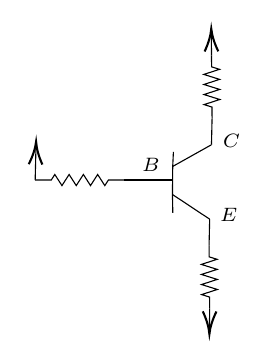
\begin{tikzpicture}[x=0.75pt,y=0.75pt,yscale=-1,xscale=1]
%uncomment if require: \path (0,300); %set diagram left start at 0, and has height of 300

%Straight Lines [id:da8761221647590739] 
\draw    (193.64,172.68) -- (193.31,179.65) -- (193.25,186.21) -- (193.18,193.17) -- (193.35,201.98) ;
%Straight Lines [id:da2640112935621488] 
\draw    (193.31,179.65) -- (211.98,169.2) ;
%Straight Lines [id:da1648370658568994] 
\draw    (193.18,193.17) -- (211.11,205.06) ;
%Straight Lines [id:da4415159270787914] 
\draw    (170.06,186.21) -- (193.25,186.21) ;
%Shape: Resistor [id:dp29441846231153623] 
\draw   (127.04,186.21) -- (134.78,186.21) -- (136.5,183.53) -- (139.94,188.88) -- (143.39,183.53) -- (146.83,188.88) -- (150.27,183.53) -- (153.71,188.88) -- (157.15,183.53) -- (160.59,188.88) -- (162.32,186.21) -- (170.06,186.21) ;
%Shape: Resistor [id:dp5088015919819379] 
\draw   (210.82,217.76) -- (210.87,223.21) -- (214.68,224.4) -- (207.1,226.86) -- (214.73,229.25) -- (207.14,231.7) -- (214.77,234.09) -- (207.19,236.55) -- (214.82,238.93) -- (207.23,241.39) -- (211.05,242.58) -- (211.1,248.03) ;
%Straight Lines [id:da9937782099239136] 
\draw    (211.11,205.06) -- (210.82,217.76) ;
%Straight Lines [id:da24739338034252478] 
\draw    (212.27,156.5) -- (211.98,169.2) ;
%Shape: Resistor [id:dp3026242553613919] 
\draw   (211.99,126.22) -- (212.04,131.67) -- (215.86,132.87) -- (208.28,135.32) -- (215.9,137.71) -- (208.32,140.17) -- (215.95,142.55) -- (208.36,145.01) -- (215.99,147.4) -- (208.41,149.86) -- (212.22,151.05) -- (212.27,156.5) ;
%Straight Lines [id:da882490167261901] 
\draw    (211.1,248.03) -- (211,258.43) ;
\draw [shift={(210.98,260.43)}, rotate = 270.54] [color={rgb, 255:red, 0; green, 0; blue, 0 }  ][line width=0.75]    (10.93,-3.29) .. controls (6.95,-1.4) and (3.31,-0.3) .. (0,0) .. controls (3.31,0.3) and (6.95,1.4) .. (10.93,3.29)   ;
%Straight Lines [id:da8615653204701303] 
\draw    (212,126.22) -- (211.9,115.3) ;
\draw [shift={(211.88,113.3)}, rotate = 89.48] [color={rgb, 255:red, 0; green, 0; blue, 0 }  ][line width=0.75]    (10.93,-3.29) .. controls (6.95,-1.4) and (3.31,-0.3) .. (0,0) .. controls (3.31,0.3) and (6.95,1.4) .. (10.93,3.29)   ;
%Straight Lines [id:da8312187874192022] 
\draw    (127.04,186.21) -- (127.44,169.74) ;
\draw [shift={(127.48,167.74)}, rotate = 91.38] [color={rgb, 255:red, 0; green, 0; blue, 0 }  ][line width=0.75]    (10.93,-3.29) .. controls (6.95,-1.4) and (3.31,-0.3) .. (0,0) .. controls (3.31,0.3) and (6.95,1.4) .. (10.93,3.29)   ;

% Text Node
\draw (216.26,162.65) node [anchor=north west][inner sep=0.75pt]  [font=\scriptsize]  {$C$};
% Text Node
\draw (177.26,174.65) node [anchor=north west][inner sep=0.75pt]  [font=\scriptsize]  {$B$};
% Text Node
\draw (214.93,198.31) node [anchor=north west][inner sep=0.75pt]  [font=\scriptsize]  {$E$};
\end{tikzpicture}
\end{center}
因為
$$
i_E = (1+\beta) i_B
$$
若把它換到 B 那邊的話就變成
$$
V_B - i_B R_B - 0.7V - (1+\beta) i_B R_E = 0
$$
若換成 E 那邊就是
$$
V_B - \frac{1}{1-\beta} i_E R_B - 0.7V - i_E R_E = 0
$$
\newpage

\section*{Small signal of BJT}
\subsection*{Basic equation}
\textbf{Transconductance:} $g_m$, 進入小訊號的鑰匙
$$
g_m \equiv \frac{I_C}{V_T}
$$
$r_{\pi}, r_e$ 的小訊號輸入電阻
\begin{align*}
	r_{\pi} \equiv \frac{\beta}{g_m} \\
	r_e \equiv \frac{\alpha}{g_m}
\end{align*}


若要求小訊號的電流都需要 $v_{be}$
\begin{align*}
	i_c = g_m v_{be} \\
	i_b = r_{\pi} v_{be} \\
	i_e = r_e v_{be}
\end{align*}

\subsection*{$\pi$ model}
$v_{be} = v_{\pi}$
\begin{center}


\tikzset{every picture/.style={line width=0.75pt}} %set default line width to 0.75pt        

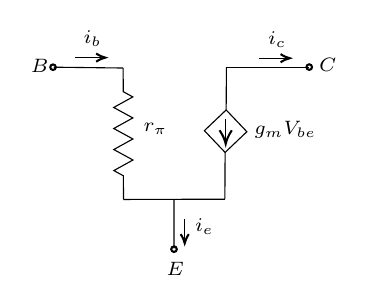
\begin{tikzpicture}[x=0.75pt,y=0.75pt,yscale=-1,xscale=1]
%uncomment if require: \path (0,300); %set diagram left start at 0, and has height of 300

%Straight Lines [id:da07178132775524226] 
\draw    (77.15,140.33) -- (110.6,140.73) ;
\draw [shift={(76.81,140.33)}, rotate = 0.68] [color={rgb, 255:red, 0; green, 0; blue, 0 }  ][line width=0.75]      (0, 0) circle [x radius= 1.34, y radius= 1.34]   ;
%Shape: Resistor [id:dp5351213227323897] 
\draw   (110.6,140.73) -- (110.63,152.13) -- (115.25,154.65) -- (106.04,159.74) -- (115.27,164.78) -- (106.06,169.87) -- (115.29,174.91) -- (106.08,180) -- (115.32,185.05) -- (106.11,190.13) -- (110.72,192.66) -- (110.75,204.06) ;
%Straight Lines [id:da41198082274172] 
\draw    (159.61,203.93) -- (135.11,203.99) -- (110.75,204.06) ;
%Shape: Square [id:dp8894047869890526] 
\draw   (160.22,160.93) -- (170.2,171.42) -- (159.71,181.39) -- (149.74,170.91) -- cycle ;
%Straight Lines [id:da39911655287248793] 
\draw    (159.71,181.39) -- (159.61,203.93) ;
%Straight Lines [id:da14140975551934143] 
\draw    (160,165.29) -- (160,175.29) ;
\draw [shift={(160,177.29)}, rotate = 270] [color={rgb, 255:red, 0; green, 0; blue, 0 }  ][line width=0.75]    (6.56,-2.94) .. controls (4.17,-1.38) and (1.99,-0.4) .. (0,0) .. controls (1.99,0.4) and (4.17,1.38) .. (6.56,2.94)   ;
%Straight Lines [id:da0839685654901382] 
\draw    (160.22,160.93) -- (160.35,140.28) ;
%Straight Lines [id:da1771382725655215] 
\draw    (160.35,140.28) -- (199.91,140.28) ;
\draw [shift={(200.25,140.28)}, rotate = 0] [color={rgb, 255:red, 0; green, 0; blue, 0 }  ][line width=0.75]      (0, 0) circle [x radius= 1.34, y radius= 1.34]   ;
%Straight Lines [id:da874147600682937] 
\draw    (135.11,203.99) -- (135.1,227.67) ;
\draw [shift={(135.1,228.01)}, rotate = 90.01] [color={rgb, 255:red, 0; green, 0; blue, 0 }  ][line width=0.75]      (0, 0) circle [x radius= 1.34, y radius= 1.34]   ;
%Straight Lines [id:da0924518057471696] 
\draw    (87.39,135.71) -- (99.96,135.71) ;
\draw [shift={(101.96,135.71)}, rotate = 180] [color={rgb, 255:red, 0; green, 0; blue, 0 }  ][line width=0.75]    (4.37,-1.96) .. controls (2.78,-0.92) and (1.32,-0.27) .. (0,0) .. controls (1.32,0.27) and (2.78,0.92) .. (4.37,1.96)   ;
%Straight Lines [id:da6667515851911453] 
\draw    (176.25,136) -- (188.82,136) ;
\draw [shift={(190.82,136)}, rotate = 180] [color={rgb, 255:red, 0; green, 0; blue, 0 }  ][line width=0.75]    (4.37,-1.96) .. controls (2.78,-0.92) and (1.32,-0.27) .. (0,0) .. controls (1.32,0.27) and (2.78,0.92) .. (4.37,1.96)   ;
%Straight Lines [id:da9368032021267306] 
\draw    (140.25,213.43) -- (140.25,223.14) ;
\draw [shift={(140.25,225.14)}, rotate = 270] [color={rgb, 255:red, 0; green, 0; blue, 0 }  ][line width=0.75]    (4.37,-1.96) .. controls (2.78,-0.92) and (1.32,-0.27) .. (0,0) .. controls (1.32,0.27) and (2.78,0.92) .. (4.37,1.96)   ;

% Text Node
\draw (119.14,165.98) node [anchor=north west][inner sep=0.75pt]  [font=\scriptsize]  {$r_{\pi }$};
% Text Node
\draw (172.57,165.13) node [anchor=north west][inner sep=0.75pt]  [font=\scriptsize]  {$g_{m} V_{be}$};
% Text Node
\draw (64.86,135.13) node [anchor=north west][inner sep=0.75pt]  [font=\scriptsize]  {$B$};
% Text Node
\draw (203.71,134.84) node [anchor=north west][inner sep=0.75pt]  [font=\scriptsize]  {$C$};
% Text Node
\draw (130.29,233.13) node [anchor=north west][inner sep=0.75pt]  [font=\scriptsize]  {$E$};
% Text Node
\draw (90.29,121.56) node [anchor=north west][inner sep=0.75pt]  [font=\scriptsize]  {$i_{b}$};
% Text Node
\draw (179.14,121.84) node [anchor=north west][inner sep=0.75pt]  [font=\scriptsize]  {$i_{c}$};
% Text Node
\draw (144,212.13) node [anchor=north west][inner sep=0.75pt]  [font=\scriptsize]  {$i_{e}$};
\end{tikzpicture}
\end{center}

\textbf{With earyly effect}
\begin{center}
	

\tikzset{every picture/.style={line width=0.75pt}} %set default line width to 0.75pt        

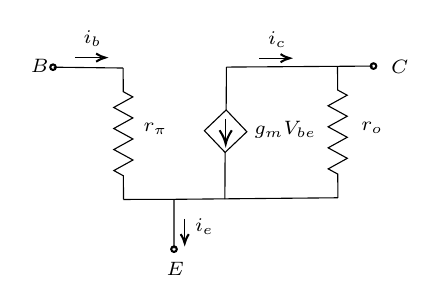
\begin{tikzpicture}[x=0.75pt,y=0.75pt,yscale=-1,xscale=1]
%uncomment if require: \path (0,300); %set diagram left start at 0, and has height of 300

%Straight Lines [id:da07178132775524226] 
\draw    (77.15,140.33) -- (110.6,140.73) ;
\draw [shift={(76.81,140.33)}, rotate = 0.68] [color={rgb, 255:red, 0; green, 0; blue, 0 }  ][line width=0.75]      (0, 0) circle [x radius= 1.34, y radius= 1.34]   ;
%Shape: Resistor [id:dp5351213227323897] 
\draw   (110.6,140.73) -- (110.63,152.13) -- (115.25,154.65) -- (106.04,159.74) -- (115.27,164.78) -- (106.06,169.87) -- (115.29,174.91) -- (106.08,180) -- (115.32,185.05) -- (106.11,190.13) -- (110.72,192.66) -- (110.75,204.06) ;
%Straight Lines [id:da41198082274172] 
\draw    (214.03,203.24) -- (135.11,203.99) -- (110.75,204.06) ;
%Shape: Square [id:dp8894047869890526] 
\draw   (160.22,160.93) -- (170.2,171.42) -- (159.71,181.39) -- (149.74,170.91) -- cycle ;
%Straight Lines [id:da39911655287248793] 
\draw    (159.71,181.39) -- (159.61,203.93) ;
%Straight Lines [id:da14140975551934143] 
\draw    (160,165.29) -- (160,175.29) ;
\draw [shift={(160,177.29)}, rotate = 270] [color={rgb, 255:red, 0; green, 0; blue, 0 }  ][line width=0.75]    (6.56,-2.94) .. controls (4.17,-1.38) and (1.99,-0.4) .. (0,0) .. controls (1.99,0.4) and (4.17,1.38) .. (6.56,2.94)   ;
%Straight Lines [id:da0839685654901382] 
\draw    (160.22,160.93) -- (160.35,140.28) ;
%Straight Lines [id:da1771382725655215] 
\draw    (160.35,140.28) -- (213.88,139.91) -- (230.87,139.79) ;
\draw [shift={(231.21,139.79)}, rotate = 359.6] [color={rgb, 255:red, 0; green, 0; blue, 0 }  ][line width=0.75]      (0, 0) circle [x radius= 1.34, y radius= 1.34]   ;
%Straight Lines [id:da874147600682937] 
\draw    (135.11,203.99) -- (135.1,227.67) ;
\draw [shift={(135.1,228.01)}, rotate = 90.01] [color={rgb, 255:red, 0; green, 0; blue, 0 }  ][line width=0.75]      (0, 0) circle [x radius= 1.34, y radius= 1.34]   ;
%Straight Lines [id:da0924518057471696] 
\draw    (87.39,135.71) -- (99.96,135.71) ;
\draw [shift={(101.96,135.71)}, rotate = 180] [color={rgb, 255:red, 0; green, 0; blue, 0 }  ][line width=0.75]    (4.37,-1.96) .. controls (2.78,-0.92) and (1.32,-0.27) .. (0,0) .. controls (1.32,0.27) and (2.78,0.92) .. (4.37,1.96)   ;
%Straight Lines [id:da6667515851911453] 
\draw    (176.25,136) -- (188.82,136) ;
\draw [shift={(190.82,136)}, rotate = 180] [color={rgb, 255:red, 0; green, 0; blue, 0 }  ][line width=0.75]    (4.37,-1.96) .. controls (2.78,-0.92) and (1.32,-0.27) .. (0,0) .. controls (1.32,0.27) and (2.78,0.92) .. (4.37,1.96)   ;
%Straight Lines [id:da9368032021267306] 
\draw    (140.25,213.43) -- (140.25,223.14) ;
\draw [shift={(140.25,225.14)}, rotate = 270] [color={rgb, 255:red, 0; green, 0; blue, 0 }  ][line width=0.75]    (4.37,-1.96) .. controls (2.78,-0.92) and (1.32,-0.27) .. (0,0) .. controls (1.32,0.27) and (2.78,0.92) .. (4.37,1.96)   ;
%Shape: Resistor [id:dp24365358771371104] 
\draw   (213.88,139.91) -- (213.91,151.31) -- (218.53,153.83) -- (209.32,158.92) -- (218.55,163.96) -- (209.34,169.05) -- (218.57,174.1) -- (209.36,179.18) -- (218.6,184.23) -- (209.39,189.32) -- (214,191.84) -- (214.03,203.24) ;

% Text Node
\draw (119.14,165.98) node [anchor=north west][inner sep=0.75pt]  [font=\scriptsize]  {$r_{\pi }$};
% Text Node
\draw (172.57,165.13) node [anchor=north west][inner sep=0.75pt]  [font=\scriptsize]  {$g_{m} V_{be}$};
% Text Node
\draw (64.86,135.13) node [anchor=north west][inner sep=0.75pt]  [font=\scriptsize]  {$B$};
% Text Node
\draw (238.38,135.51) node [anchor=north west][inner sep=0.75pt]  [font=\scriptsize]  {$C$};
% Text Node
\draw (130.29,233.13) node [anchor=north west][inner sep=0.75pt]  [font=\scriptsize]  {$E$};
% Text Node
\draw (90.29,121.56) node [anchor=north west][inner sep=0.75pt]  [font=\scriptsize]  {$i_{b}$};
% Text Node
\draw (179.14,121.84) node [anchor=north west][inner sep=0.75pt]  [font=\scriptsize]  {$i_{c}$};
% Text Node
\draw (144,212.13) node [anchor=north west][inner sep=0.75pt]  [font=\scriptsize]  {$i_{e}$};
% Text Node
\draw (224.14,165.48) node [anchor=north west][inner sep=0.75pt]  [font=\scriptsize]  {$r_{o}$};
\end{tikzpicture}
\end{center}
\newpage

\subsection*{T model}
$v_{be} = v_{\pi}$
\begin{center}
	

\tikzset{every picture/.style={line width=0.75pt}} %set default line width to 0.75pt        

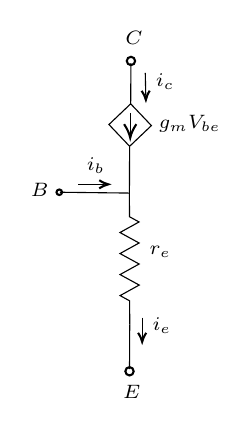
\begin{tikzpicture}[x=0.75pt,y=0.75pt,yscale=-1,xscale=1]
%uncomment if require: \path (0,300); %set diagram left start at 0, and has height of 300

%Straight Lines [id:da07178132775524226] 
\draw    (94.66,129.03) -- (128.11,129.43) ;
\draw [shift={(94.32,129.03)}, rotate = 0.68] [color={rgb, 255:red, 0; green, 0; blue, 0 }  ][line width=0.75]      (0, 0) circle [x radius= 1.34, y radius= 1.34]   ;
%Shape: Resistor [id:dp5351213227323897] 
\draw   (128.11,129.43) -- (128.14,140.83) -- (132.76,143.35) -- (123.55,148.44) -- (132.78,153.48) -- (123.57,158.57) -- (132.8,163.61) -- (123.59,168.7) -- (132.83,173.75) -- (123.62,178.83) -- (128.23,181.36) -- (128.26,192.76) ;
%Shape: Square [id:dp8894047869890526] 
\draw   (128.72,86.43) -- (138.7,96.92) -- (128.21,106.89) -- (118.24,96.41) -- cycle ;
%Straight Lines [id:da39911655287248793] 
\draw    (128.21,106.89) -- (128.11,129.43) ;
%Straight Lines [id:da14140975551934143] 
\draw    (128.5,90.79) -- (128.5,100.79) ;
\draw [shift={(128.5,102.79)}, rotate = 270] [color={rgb, 255:red, 0; green, 0; blue, 0 }  ][line width=0.75]    (6.56,-2.94) .. controls (4.17,-1.38) and (1.99,-0.4) .. (0,0) .. controls (1.99,0.4) and (4.17,1.38) .. (6.56,2.94)   ;
%Straight Lines [id:da0839685654901382] 
\draw    (128.72,86.43) -- (128.84,66.79) ;
\draw [shift={(128.85,65.78)}, rotate = 270.35] [color={rgb, 255:red, 0; green, 0; blue, 0 }  ][line width=0.75]      (0, 0) circle [x radius= 2.01, y radius= 2.01]   ;
%Straight Lines [id:da0924518057471696] 
\draw    (103.39,125.21) -- (115.96,125.21) ;
\draw [shift={(117.96,125.21)}, rotate = 180] [color={rgb, 255:red, 0; green, 0; blue, 0 }  ][line width=0.75]    (4.37,-1.96) .. controls (2.78,-0.92) and (1.32,-0.27) .. (0,0) .. controls (1.32,0.27) and (2.78,0.92) .. (4.37,1.96)   ;
%Straight Lines [id:da6667515851911453] 
\draw    (135.75,71.5) -- (135.99,82.51) ;
\draw [shift={(136.04,84.51)}, rotate = 268.71] [color={rgb, 255:red, 0; green, 0; blue, 0 }  ][line width=0.75]    (4.37,-1.96) .. controls (2.78,-0.92) and (1.32,-0.27) .. (0,0) .. controls (1.32,0.27) and (2.78,0.92) .. (4.37,1.96)   ;
%Straight Lines [id:da9368032021267306] 
\draw    (134.25,189.43) -- (134.25,199.14) ;
\draw [shift={(134.25,201.14)}, rotate = 270] [color={rgb, 255:red, 0; green, 0; blue, 0 }  ][line width=0.75]    (4.37,-1.96) .. controls (2.78,-0.92) and (1.32,-0.27) .. (0,0) .. controls (1.32,0.27) and (2.78,0.92) .. (4.37,1.96)   ;
%Straight Lines [id:da34359585028837325] 
\draw    (128.26,192.76) -- (128.16,214.28) ;
\draw [shift={(128.16,215.29)}, rotate = 90.25] [color={rgb, 255:red, 0; green, 0; blue, 0 }  ][line width=0.75]      (0, 0) circle [x radius= 2.01, y radius= 2.01]   ;

% Text Node
\draw (136.64,153.98) node [anchor=north west][inner sep=0.75pt]  [font=\scriptsize]  {$r_{e}$};
% Text Node
\draw (141.07,90.63) node [anchor=north west][inner sep=0.75pt]  [font=\scriptsize]  {$g_{m} V_{be}$};
% Text Node
\draw (79.36,123.63) node [anchor=north west][inner sep=0.75pt]  [font=\scriptsize]  {$B$};
% Text Node
\draw (124.88,50.01) node [anchor=north west][inner sep=0.75pt]  [font=\scriptsize]  {$C$};
% Text Node
\draw (123.79,220.63) node [anchor=north west][inner sep=0.75pt]  [font=\scriptsize]  {$E$};
% Text Node
\draw (106.29,111.06) node [anchor=north west][inner sep=0.75pt]  [font=\scriptsize]  {$i_{b}$};
% Text Node
\draw (139.64,70.84) node [anchor=north west][inner sep=0.75pt]  [font=\scriptsize]  {$i_{c}$};
% Text Node
\draw (138,188.13) node [anchor=north west][inner sep=0.75pt]  [font=\scriptsize]  {$i_{e}$};
\end{tikzpicture}
\end{center}

\textbf{With earyly effect}
\begin{center}
  

\tikzset{every picture/.style={line width=0.75pt}} %set default line width to 0.75pt        

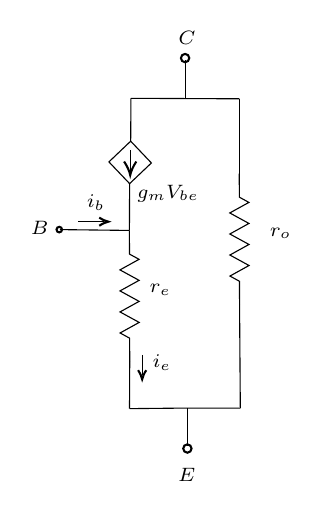
\begin{tikzpicture}[x=0.75pt,y=0.75pt,yscale=-1,xscale=1]
%uncomment if require: \path (0,300); %set diagram left start at 0, and has height of 300

%Straight Lines [id:da07178132775524226] 
\draw    (94.66,129.03) -- (128.11,129.43) ;
\draw [shift={(94.32,129.03)}, rotate = 0.68] [color={rgb, 255:red, 0; green, 0; blue, 0 }  ][line width=0.75]      (0, 0) circle [x radius= 1.34, y radius= 1.34]   ;
%Shape: Resistor [id:dp5351213227323897] 
\draw   (128.11,129.43) -- (128.14,140.83) -- (132.76,143.35) -- (123.55,148.44) -- (132.78,153.48) -- (123.57,158.57) -- (132.8,163.61) -- (123.59,168.7) -- (132.83,173.75) -- (123.62,178.83) -- (128.23,181.36) -- (128.26,192.76) ;
%Shape: Square [id:dp8894047869890526] 
\draw   (128.72,86.43) -- (138.7,96.92) -- (128.21,106.89) -- (118.24,96.41) -- cycle ;
%Straight Lines [id:da39911655287248793] 
\draw    (128.21,106.89) -- (128.11,129.43) ;
%Straight Lines [id:da14140975551934143] 
\draw    (128.5,90.79) -- (128.5,100.79) ;
\draw [shift={(128.5,102.79)}, rotate = 270] [color={rgb, 255:red, 0; green, 0; blue, 0 }  ][line width=0.75]    (6.56,-2.94) .. controls (4.17,-1.38) and (1.99,-0.4) .. (0,0) .. controls (1.99,0.4) and (4.17,1.38) .. (6.56,2.94)   ;
%Straight Lines [id:da0839685654901382] 
\draw    (128.72,86.43) -- (128.85,65.78) ;
%Straight Lines [id:da0924518057471696] 
\draw    (103.39,125.21) -- (115.96,125.21) ;
\draw [shift={(117.96,125.21)}, rotate = 180] [color={rgb, 255:red, 0; green, 0; blue, 0 }  ][line width=0.75]    (4.37,-1.96) .. controls (2.78,-0.92) and (1.32,-0.27) .. (0,0) .. controls (1.32,0.27) and (2.78,0.92) .. (4.37,1.96)   ;
%Straight Lines [id:da9368032021267306] 
\draw    (134.25,189.43) -- (134.25,199.14) ;
\draw [shift={(134.25,201.14)}, rotate = 270] [color={rgb, 255:red, 0; green, 0; blue, 0 }  ][line width=0.75]    (4.37,-1.96) .. controls (2.78,-0.92) and (1.32,-0.27) .. (0,0) .. controls (1.32,0.27) and (2.78,0.92) .. (4.37,1.96)   ;
%Straight Lines [id:da34359585028837325] 
\draw    (128.26,192.76) -- (128.16,215.29) ;
%Straight Lines [id:da11042212161425502] 
\draw    (128.85,65.78) -- (181.04,66.01) ;
%Shape: Resistor [id:dp21389434232783167] 
\draw   (181.04,102.01) -- (181.07,113.4) -- (185.68,115.93) -- (176.47,121.01) -- (185.7,126.06) -- (176.49,131.15) -- (185.73,136.19) -- (176.52,141.28) -- (185.75,146.33) -- (176.54,151.41) -- (181.16,153.94) -- (181.18,165.34) ;
%Straight Lines [id:da6528634062643753] 
\draw    (181.04,102.01) -- (181.04,66.01) ;
%Straight Lines [id:da4415370273417265] 
\draw    (128.16,215.29) -- (156.04,215.01) -- (181.54,215.01) ;
%Straight Lines [id:da6151262814661648] 
\draw    (181.54,215.01) -- (181.18,165.34) ;
%Straight Lines [id:da6590118212280813] 
\draw    (156.04,215.01) -- (156.04,233.5) ;
\draw [shift={(156.04,234.51)}, rotate = 90] [color={rgb, 255:red, 0; green, 0; blue, 0 }  ][line width=0.75]      (0, 0) circle [x radius= 2.01, y radius= 2.01]   ;
%Straight Lines [id:da1996809266577637] 
\draw    (154.94,47.4) -- (154.94,65.89) ;
\draw [shift={(154.94,46.39)}, rotate = 90] [color={rgb, 255:red, 0; green, 0; blue, 0 }  ][line width=0.75]      (0, 0) circle [x radius= 2.01, y radius= 2.01]   ;

% Text Node
\draw (136.64,153.98) node [anchor=north west][inner sep=0.75pt]  [font=\scriptsize]  {$r_{e}$};
% Text Node
\draw (130.5,106.19) node [anchor=north west][inner sep=0.75pt]  [font=\scriptsize]  {$g_{m} V_{be}$};
% Text Node
\draw (79.36,123.63) node [anchor=north west][inner sep=0.75pt]  [font=\scriptsize]  {$B$};
% Text Node
\draw (150.38,32.01) node [anchor=north west][inner sep=0.75pt]  [font=\scriptsize]  {$C$};
% Text Node
\draw (150.29,242.63) node [anchor=north west][inner sep=0.75pt]  [font=\scriptsize]  {$E$};
% Text Node
\draw (106.29,111.06) node [anchor=north west][inner sep=0.75pt]  [font=\scriptsize]  {$i_{b}$};
% Text Node
\draw (138,188.13) node [anchor=north west][inner sep=0.75pt]  [font=\scriptsize]  {$i_{e}$};
% Text Node
\draw (194.5,126.9) node [anchor=north west][inner sep=0.75pt]  [font=\scriptsize]  {$r_{o}$};
\end{tikzpicture}
\end{center}

\newpage
\section*{Amplify of BJT}
\subsection*{Common Emmiter (CE)}
\begin{center}


\tikzset{every picture/.style={line width=0.75pt}} %set default line width to 0.75pt        

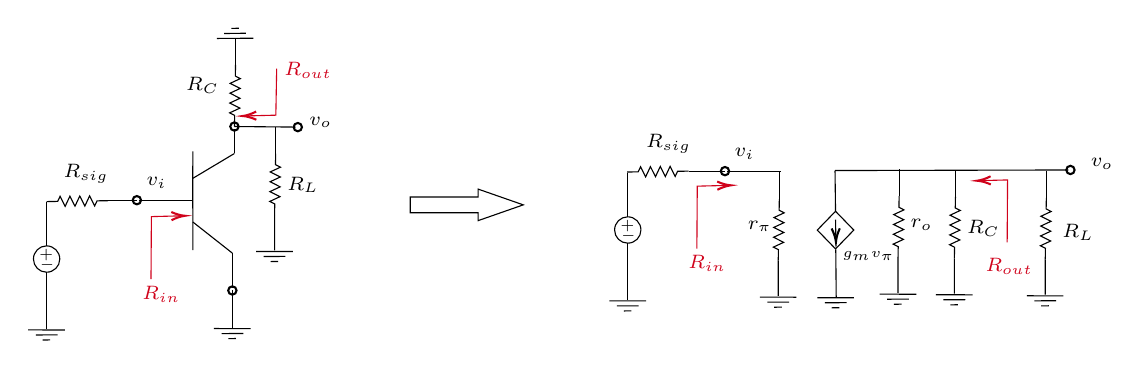
\begin{tikzpicture}[x=0.75pt,y=0.75pt,yscale=-1,xscale=1]
%uncomment if require: \path (0,300); %set diagram left start at 0, and has height of 300

%Straight Lines [id:da4133500324477516] 
\draw    (110.6,100.31) -- (110.49,113.32) -- (110.53,123.81) -- (110.56,134.31) -- (110.6,147.81) ;
%Straight Lines [id:da7830670584441963] 
\draw    (110.49,113.32) -- (130.6,101.31) ;
%Straight Lines [id:da30721918777675417] 
\draw    (110.56,134.31) -- (129.6,149.31) ;
%Straight Lines [id:da9997255942735996] 
\draw    (84.61,123.81) -- (110.53,123.81) ;
\draw [shift={(83.6,123.81)}, rotate = 359.99] [color={rgb, 255:red, 0; green, 0; blue, 0 }  ][line width=0.75]      (0, 0) circle [x radius= 2.01, y radius= 2.01]   ;
%Straight Lines [id:da43133315122711613] 
\draw    (130.6,101.31) -- (130.6,89.32) ;
\draw [shift={(130.6,88.31)}, rotate = 270] [color={rgb, 255:red, 0; green, 0; blue, 0 }  ][line width=0.75]      (0, 0) circle [x radius= 2.01, y radius= 2.01]   ;
%Straight Lines [id:da8942046760449994] 
\draw    (129.6,149.31) -- (129.6,166.3) ;
\draw [shift={(129.6,167.31)}, rotate = 90] [color={rgb, 255:red, 0; green, 0; blue, 0 }  ][line width=0.75]      (0, 0) circle [x radius= 2.01, y radius= 2.01]   ;
%Straight Lines [id:da8684535561057921] 
\draw    (129.6,167.31) -- (129.6,185.31) ;
%Straight Lines [id:da45977051079735065] 
\draw    (66.1,123.81) -- (83.6,123.81) ;
%Straight Lines [id:da7275933354176902] 
\draw    (40.1,124.48) -- (40.1,145.82) ;
%Shape: Circle [id:dp9764375079104787] 
\draw   (33.76,152.17) .. controls (33.76,148.66) and (36.6,145.82) .. (40.1,145.82) .. controls (43.61,145.82) and (46.45,148.66) .. (46.45,152.17) .. controls (46.45,155.67) and (43.61,158.51) .. (40.1,158.51) .. controls (36.6,158.51) and (33.76,155.67) .. (33.76,152.17) -- cycle ;
%Straight Lines [id:da3845153328683255] 
\draw    (40.1,158.51) -- (40.1,185.82) ;
%Straight Lines [id:da46423949264715025] 
\draw    (34.9,188.75) -- (45.38,188.7) ;
%Straight Lines [id:da5793601408315048] 
\draw    (38.19,191.18) -- (41.85,191.13) ;
%Straight Lines [id:da9878557919971883] 
\draw    (31.25,186.31) -- (48.92,186.35) ;

%Straight Lines [id:da5914914926844957] 
\draw    (124.4,188.08) -- (134.88,188.03) ;
%Straight Lines [id:da09483804649922112] 
\draw    (127.69,190.51) -- (131.35,190.46) ;
%Straight Lines [id:da5122315853274279] 
\draw    (120.75,185.65) -- (138.42,185.68) ;

%Shape: Resistor [id:dp14873311531817002] 
\draw   (131.13,58.67) -- (131.04,64) -- (133.46,65.23) -- (128.53,67.51) -- (133.38,69.97) -- (128.44,72.26) -- (133.29,74.72) -- (128.36,77) -- (133.21,79.46) -- (128.28,81.74) -- (130.7,82.97) -- (130.6,88.31) ;
%Straight Lines [id:da2938292496744518] 
\draw    (131.13,58.67) -- (131.13,45.67) ;
%Straight Lines [id:da20941830503677983] 
\draw    (136.1,43.37) -- (125.61,43.51) ;
%Straight Lines [id:da11007517241569709] 
\draw    (132.78,40.96) -- (129.12,41.04) ;
%Straight Lines [id:da6538432568343695] 
\draw    (139.77,45.77) -- (122.1,45.89) ;

%Straight Lines [id:da05635601673206281] 
\draw    (130.6,88.31) -- (160.12,88.59) ;
\draw [shift={(161.13,88.6)}, rotate = 0.55] [color={rgb, 255:red, 0; green, 0; blue, 0 }  ][line width=0.75]      (0, 0) circle [x radius= 2.01, y radius= 2.01]   ;
%Right Arrow [id:dp979410899189834] 
\draw   (215.33,122.26) -- (247.99,122.26) -- (247.99,118.46) -- (269.76,126.06) -- (247.99,133.67) -- (247.99,129.86) -- (215.33,129.86) -- cycle ;
%Straight Lines [id:da31447814252608675] 
\draw    (367.95,109.81) -- (393.86,109.81) ;
\draw [shift={(366.94,109.81)}, rotate = 359.99] [color={rgb, 255:red, 0; green, 0; blue, 0 }  ][line width=0.75]      (0, 0) circle [x radius= 2.01, y radius= 2.01]   ;
%Straight Lines [id:da12840167180127693] 
\draw    (349.44,109.81) -- (366.94,109.81) ;
%Straight Lines [id:da9613612391720225] 
\draw    (320.1,110.48) -- (320.1,131.82) ;
%Shape: Circle [id:dp11668143109232387] 
\draw   (313.76,138.17) .. controls (313.76,134.66) and (316.6,131.82) .. (320.1,131.82) .. controls (323.61,131.82) and (326.45,134.66) .. (326.45,138.17) .. controls (326.45,141.67) and (323.61,144.51) .. (320.1,144.51) .. controls (316.6,144.51) and (313.76,141.67) .. (313.76,138.17) -- cycle ;
%Straight Lines [id:da6726527399127464] 
\draw    (320.1,144.51) -- (320.1,171.82) ;
%Straight Lines [id:da2636135648161585] 
\draw    (314.9,174.75) -- (325.38,174.7) ;
%Straight Lines [id:da7358310616474298] 
\draw    (318.19,177.18) -- (321.85,177.13) ;
%Straight Lines [id:da9497899944455356] 
\draw    (311.25,172.31) -- (328.92,172.35) ;

%Shape: Resistor [id:dp43577407497286336] 
\draw   (393.13,123.33) -- (393.04,128.67) -- (395.46,129.9) -- (390.53,132.18) -- (395.38,134.64) -- (390.44,136.92) -- (395.29,139.38) -- (390.36,141.67) -- (395.21,144.13) -- (390.28,146.41) -- (392.7,147.64) -- (392.6,152.98) ;
%Straight Lines [id:da6799746466189092] 
\draw    (393.13,123.33) -- (393.13,110.33) ;
%Straight Lines [id:da6899976724461269] 
\draw    (392.6,152.98) -- (392.59,169.95) ;
%Straight Lines [id:da46577040538889314] 
\draw    (387.36,172.95) -- (397.85,172.9) ;
%Straight Lines [id:da5885793414894771] 
\draw    (390.66,175.38) -- (394.32,175.33) ;
%Straight Lines [id:da7386724632814998] 
\draw    (383.72,170.51) -- (401.38,170.55) ;

%Flowchart: Decision [id:dp33499331630798135] 
\draw   (420.21,129.15) -- (429.01,138.21) -- (420.21,147.27) -- (411.41,138.21) -- cycle ;
%Straight Lines [id:da29171091451254105] 
\draw    (420.21,133.23) -- (420.36,141.98) ;
\draw [shift={(420.4,143.98)}, rotate = 269.03] [color={rgb, 255:red, 0; green, 0; blue, 0 }  ][line width=0.75]    (6.56,-1.97) .. controls (4.17,-0.84) and (1.99,-0.18) .. (0,0) .. controls (1.99,0.18) and (4.17,0.84) .. (6.56,1.97)   ;
%Straight Lines [id:da07311807614415755] 
\draw    (420.21,129.15) -- (419.96,109.53) ;
%Straight Lines [id:da4775554430514444] 
\draw    (419.96,109.53) -- (532.37,109.25) ;
\draw [shift={(533.38,109.25)}, rotate = 359.86] [color={rgb, 255:red, 0; green, 0; blue, 0 }  ][line width=0.75]      (0, 0) circle [x radius= 2.01, y radius= 2.01]   ;
%Straight Lines [id:da8191452432814792] 
\draw    (420.32,147.55) -- (420.53,170.39) ;
%Straight Lines [id:da8170178406378605] 
\draw    (415.08,173.23) -- (425.56,173.18) ;
%Straight Lines [id:da5247965928086409] 
\draw    (418.37,175.66) -- (422.03,175.62) ;
%Straight Lines [id:da30929355421800153] 
\draw    (411.43,170.8) -- (429.1,170.83) ;

%Shape: Resistor [id:dp4480904678351729] 
\draw   (450.85,121.9) -- (450.75,127.24) -- (453.18,128.47) -- (448.24,130.75) -- (453.09,133.21) -- (448.16,135.5) -- (453.01,137.95) -- (448.07,140.24) -- (452.92,142.7) -- (447.99,144.98) -- (450.41,146.21) -- (450.32,151.55) ;
%Straight Lines [id:da531862362567862] 
\draw    (450.85,121.9) -- (450.85,108.9) ;
%Straight Lines [id:da7382081507976663] 
\draw    (450.32,151.55) -- (450.31,168.52) ;
%Straight Lines [id:da5196062565986387] 
\draw    (445.08,171.52) -- (455.56,171.47) ;
%Straight Lines [id:da8927945578099123] 
\draw    (448.37,173.95) -- (452.03,173.9) ;
%Straight Lines [id:da9736886629701076] 
\draw    (441.43,169.08) -- (459.1,169.12) ;

%Shape: Resistor [id:dp8037821018730359] 
\draw   (477.99,122.19) -- (477.89,127.52) -- (480.32,128.75) -- (475.39,131.04) -- (480.23,133.5) -- (475.3,135.78) -- (480.15,138.24) -- (475.22,140.53) -- (480.07,142.98) -- (475.13,145.27) -- (477.56,146.5) -- (477.46,151.83) ;
%Straight Lines [id:da9697617559311217] 
\draw    (477.99,122.19) -- (477.99,109.19) ;
%Straight Lines [id:da5158733902596043] 
\draw    (477.46,151.83) -- (477.45,168.81) ;
%Straight Lines [id:da31446650723116776] 
\draw    (472.22,171.8) -- (482.71,171.75) ;
%Straight Lines [id:da09396637551880294] 
\draw    (475.52,174.24) -- (479.18,174.19) ;
%Straight Lines [id:da13383091403857972] 
\draw    (468.57,169.37) -- (486.24,169.4) ;

%Shape: Resistor [id:dp554643998780704] 
\draw   (521.78,122.69) -- (521.68,128.02) -- (524.1,129.25) -- (519.17,131.54) -- (524.02,134) -- (519.09,136.28) -- (523.94,138.74) -- (519,141.03) -- (523.85,143.48) -- (518.92,145.77) -- (521.34,147) -- (521.25,152.33) ;
%Straight Lines [id:da09176120356550421] 
\draw    (521.78,122.69) -- (521.78,109.69) ;
%Straight Lines [id:da9274343994505203] 
\draw    (521.25,152.33) -- (521.24,169.31) ;
%Straight Lines [id:da9475171227617633] 
\draw    (516.01,172.3) -- (526.49,172.25) ;
%Straight Lines [id:da0032585860551483936] 
\draw    (519.3,174.74) -- (522.96,174.69) ;
%Straight Lines [id:da7958479005124568] 
\draw    (512.36,169.87) -- (530.02,169.9) ;

%Shape: Resistor [id:dp8231402567940131] 
\draw   (319.79,110.24) -- (325.13,110.16) -- (326.28,107.7) -- (328.72,112.56) -- (331.02,107.63) -- (333.46,112.49) -- (335.77,107.56) -- (338.21,112.42) -- (340.51,107.49) -- (342.95,112.35) -- (344.1,109.89) -- (349.44,109.81) ;
%Shape: Resistor [id:dp5073701885339131] 
\draw   (40.1,124.48) -- (45.44,124.4) -- (46.59,121.94) -- (49.03,126.79) -- (51.33,121.87) -- (53.78,126.72) -- (56.08,121.8) -- (58.52,126.66) -- (60.82,121.73) -- (63.26,126.59) -- (64.41,124.12) -- (69.75,124.05) ;
%Shape: Resistor [id:dp8922314605853572] 
\draw   (150.47,101.33) -- (150.37,106.67) -- (152.8,107.9) -- (147.86,110.18) -- (152.71,112.64) -- (147.78,114.92) -- (152.63,117.38) -- (147.69,119.67) -- (152.54,122.13) -- (147.61,124.41) -- (150.03,125.64) -- (149.94,130.98) ;
%Straight Lines [id:da7717953183916427] 
\draw    (150.47,101.33) -- (150.47,88.33) ;
%Straight Lines [id:da9116408108693664] 
\draw    (149.94,130.98) -- (149.93,147.95) ;
%Straight Lines [id:da33547757029464287] 
\draw    (144.7,150.95) -- (155.18,150.9) ;
%Straight Lines [id:da5163419418114911] 
\draw    (147.99,153.38) -- (151.65,153.33) ;
%Straight Lines [id:da09818490248088263] 
\draw    (141.05,148.51) -- (158.72,148.55) ;

%Straight Lines [id:da20174931264036466] 
\draw [color={rgb, 255:red, 208; green, 2; blue, 27 }  ,draw opacity=1 ]   (90.4,161.86) -- (90.59,131.72) -- (104.79,131.36) ;
\draw [shift={(106.79,131.32)}, rotate = 178.59] [color={rgb, 255:red, 208; green, 2; blue, 27 }  ,draw opacity=1 ][line width=0.75]    (6.56,-1.97) .. controls (4.17,-0.84) and (1.99,-0.18) .. (0,0) .. controls (1.99,0.18) and (4.17,0.84) .. (6.56,1.97)   ;
%Straight Lines [id:da06096463918473072] 
\draw [color={rgb, 255:red, 208; green, 2; blue, 27 }  ,draw opacity=1 ]   (150.95,60.45) -- (150.55,82.85) -- (136.55,83.2) ;
\draw [shift={(134.55,83.25)}, rotate = 358.57] [color={rgb, 255:red, 208; green, 2; blue, 27 }  ,draw opacity=1 ][line width=0.75]    (6.56,-1.97) .. controls (4.17,-0.84) and (1.99,-0.18) .. (0,0) .. controls (1.99,0.18) and (4.17,0.84) .. (6.56,1.97)   ;
%Straight Lines [id:da933603689262295] 
\draw [color={rgb, 255:red, 208; green, 2; blue, 27 }  ,draw opacity=1 ]   (353.4,147.19) -- (353.59,117.05) -- (367.79,116.7) ;
\draw [shift={(369.79,116.65)}, rotate = 178.59] [color={rgb, 255:red, 208; green, 2; blue, 27 }  ,draw opacity=1 ][line width=0.75]    (6.56,-1.97) .. controls (4.17,-0.84) and (1.99,-0.18) .. (0,0) .. controls (1.99,0.18) and (4.17,0.84) .. (6.56,1.97)   ;
%Straight Lines [id:da40351954903218834] 
\draw [color={rgb, 255:red, 208; green, 2; blue, 27 }  ,draw opacity=1 ]   (502.9,144.19) -- (503.09,114.05) -- (490.41,114.37) ;
\draw [shift={(488.41,114.43)}, rotate = 358.53] [color={rgb, 255:red, 208; green, 2; blue, 27 }  ,draw opacity=1 ][line width=0.75]    (6.56,-1.97) .. controls (4.17,-0.84) and (1.99,-0.18) .. (0,0) .. controls (1.99,0.18) and (4.17,0.84) .. (6.56,1.97)   ;

% Text Node
\draw (35.22,146.39) node [anchor=north west][inner sep=0.75pt]  [font=\tiny]  {$+$};
% Text Node
\draw (35.48,151.1) node [anchor=north west][inner sep=0.75pt]  [font=\tiny]  {$-$};
% Text Node
\draw (87,111.4) node [anchor=north west][inner sep=0.75pt]  [font=\scriptsize]  {$v_{i}$};
% Text Node
\draw (165.5,82.4) node [anchor=north west][inner sep=0.75pt]  [font=\scriptsize]  {$v_{o}$};
% Text Node
\draw (315.22,132.39) node [anchor=north west][inner sep=0.75pt]  [font=\tiny]  {$+$};
% Text Node
\draw (315.48,137.1) node [anchor=north west][inner sep=0.75pt]  [font=\tiny]  {$-$};
% Text Node
\draw (370.33,97.4) node [anchor=north west][inner sep=0.75pt]  [font=\scriptsize]  {$v_{i}$};
% Text Node
\draw (376.74,132.47) node [anchor=north west][inner sep=0.75pt]  [font=\scriptsize]  {$r_{\pi }$};
% Text Node
\draw (422.4,147.38) node [anchor=north west][inner sep=0.75pt]  [font=\tiny]  {$g_{m} v_{\pi }$};
% Text Node
\draw (455.18,131.87) node [anchor=north west][inner sep=0.75pt]  [font=\scriptsize]  {$r_{o}$};
% Text Node
\draw (482.32,132.15) node [anchor=north west][inner sep=0.75pt]  [font=\scriptsize]  {$R_{C}$};
% Text Node
\draw (528.22,134.25) node [anchor=north west][inner sep=0.75pt]  [font=\scriptsize]  {$R_{L}$};
% Text Node
\draw (541.94,102.27) node [anchor=north west][inner sep=0.75pt]  [font=\scriptsize]  {$v_{o}$};
% Text Node
\draw (327.65,90.66) node [anchor=north west][inner sep=0.75pt]  [font=\scriptsize]  {$R_{sig}$};
% Text Node
\draw (46.99,105.33) node [anchor=north west][inner sep=0.75pt]  [font=\scriptsize]  {$R_{sig}$};
% Text Node
\draw (106.04,63.49) node [anchor=north west][inner sep=0.75pt]  [font=\scriptsize]  {$R_{C}$};
% Text Node
\draw (154.8,111.3) node [anchor=north west][inner sep=0.75pt]  [font=\scriptsize]  {$R_{L}$};
% Text Node
\draw (85.03,163.89) node [anchor=north west][inner sep=0.75pt]  [font=\scriptsize,color={rgb, 255:red, 208; green, 2; blue, 27 }  ,opacity=1 ]  {$R_{in}$};
% Text Node
\draw (153.43,56.29) node [anchor=north west][inner sep=0.75pt]  [font=\scriptsize,color={rgb, 255:red, 208; green, 2; blue, 27 }  ,opacity=1 ]  {$R_{out}$};
% Text Node
\draw (348.03,149.22) node [anchor=north west][inner sep=0.75pt]  [font=\scriptsize,color={rgb, 255:red, 208; green, 2; blue, 27 }  ,opacity=1 ]  {$R_{in}$};
% Text Node
\draw (491.2,150.56) node [anchor=north west][inner sep=0.75pt]  [font=\scriptsize,color={rgb, 255:red, 208; green, 2; blue, 27 }  ,opacity=1 ]  {$R_{out}$};
\end{tikzpicture}
\end{center}

計算 $A_v \equiv \frac{v_o}{v_i}$
\begin{align*}
	\because   v_i &= v_\pi \\
	           v_o &= -g_m v_i (R_C || R_L) \\
	\therefore A_v &= -g_m (R_C || R_L)
\end{align*}

計算 $G_v \equiv \frac{v_{\text{sig}}} {v_o}$
\begin{align*}
	\because v_i &= v_{\text{sig}} \frac{r_{\pi}}{R_{\text{sig}} r_{\pi}} \\
	\therefore G_v &= \frac{r_{\pi}}{R_{\text{sig}} r_{\pi}} A_v
\end{align*}

\textbf{Summary of CE Amp.} \\
\begin{center}
	\begin{minipage}{0.6\textwidth}
		\begin{enumerate}[label=\arabic*.]
		  \item $\because R_{\text{in}} = r_{\pi} = \frac{\beta}{g_m}, \quad \therefore R_{\text{in}}$ 輸入阻抗沒有很高,理想的 Amp. 是$R_{\text{in}}$高; $R_{\text{out}}$低 \\
			\item $A_v = \textcolor{red} - \textcolor{black} g_m (R_C || R_L)$, 相位差了$180^{\circ}$
		\end{enumerate}
	\end{minipage}
\end{center}
\newpage

\subsection*{Common Base (CB)}
\begin{center}
	

\tikzset{every picture/.style={line width=0.75pt}} %set default line width to 0.75pt        

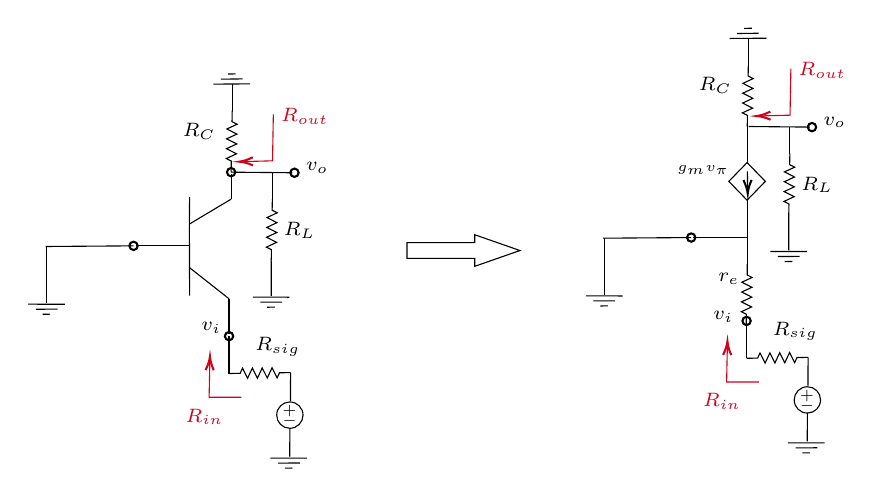
\begin{tikzpicture}[x=0.75pt,y=0.75pt,yscale=-1,xscale=1]
%uncomment if require: \path (0,300); %set diagram left start at 0, and has height of 300

%Straight Lines [id:da4133500324477516] 
\draw    (110.6,100.31) -- (110.49,113.32) -- (110.53,123.81) -- (110.56,134.31) -- (110.6,147.81) ;
%Straight Lines [id:da7830670584441963] 
\draw    (110.49,113.32) -- (130.6,101.31) ;
%Straight Lines [id:da30721918777675417] 
\draw    (110.56,134.31) -- (129.6,149.31) ;
%Straight Lines [id:da9997255942735996] 
\draw    (84.61,123.81) -- (110.53,123.81) ;
\draw [shift={(83.6,123.81)}, rotate = 359.99] [color={rgb, 255:red, 0; green, 0; blue, 0 }  ][line width=0.75]      (0, 0) circle [x radius= 2.01, y radius= 2.01]   ;
%Straight Lines [id:da43133315122711613] 
\draw    (130.6,101.31) -- (130.6,89.32) ;
\draw [shift={(130.6,88.31)}, rotate = 270] [color={rgb, 255:red, 0; green, 0; blue, 0 }  ][line width=0.75]      (0, 0) circle [x radius= 2.01, y radius= 2.01]   ;
%Straight Lines [id:da8942046760449994] 
\draw    (129.6,149.31) -- (129.6,166.3) ;
\draw [shift={(129.6,167.31)}, rotate = 90] [color={rgb, 255:red, 0; green, 0; blue, 0 }  ][line width=0.75]      (0, 0) circle [x radius= 2.01, y radius= 2.01]   ;
%Straight Lines [id:da8684535561057921] 
\draw    (129.6,167.31) -- (129.6,185.31) ;
%Straight Lines [id:da45977051079735065] 
\draw    (41.2,124.12) -- (83.6,123.81) ;
%Shape: Circle [id:dp9764375079104787] 
\draw   (152.56,205.37) .. controls (152.56,201.86) and (155.4,199.02) .. (158.9,199.02) .. controls (162.41,199.02) and (165.25,201.86) .. (165.25,205.37) .. controls (165.25,208.87) and (162.41,211.71) .. (158.9,211.71) .. controls (155.4,211.71) and (152.56,208.87) .. (152.56,205.37) -- cycle ;
%Straight Lines [id:da3845153328683255] 
\draw    (41.7,124.11) -- (41.7,151.42) ;
%Straight Lines [id:da46423949264715025] 
\draw    (36.5,154.35) -- (46.98,154.3) ;
%Straight Lines [id:da5793601408315048] 
\draw    (39.79,156.78) -- (43.45,156.73) ;
%Straight Lines [id:da9878557919971883] 
\draw    (32.85,151.91) -- (50.52,151.95) ;

%Straight Lines [id:da5914914926844957] 
\draw    (153.2,228.48) -- (163.68,228.43) ;
%Straight Lines [id:da09483804649922112] 
\draw    (156.49,230.91) -- (160.15,230.86) ;
%Straight Lines [id:da5122315853274279] 
\draw    (149.55,226.05) -- (167.22,226.08) ;

%Shape: Resistor [id:dp14873311531817002] 
\draw   (131.13,58.67) -- (131.04,64) -- (133.46,65.23) -- (128.53,67.51) -- (133.38,69.97) -- (128.44,72.26) -- (133.29,74.72) -- (128.36,77) -- (133.21,79.46) -- (128.28,81.74) -- (130.7,82.97) -- (130.6,88.31) ;
%Straight Lines [id:da2938292496744518] 
\draw    (131.13,58.67) -- (131.13,45.67) ;
%Straight Lines [id:da20941830503677983] 
\draw    (136.1,43.37) -- (125.61,43.51) ;
%Straight Lines [id:da11007517241569709] 
\draw    (132.78,40.96) -- (129.12,41.04) ;
%Straight Lines [id:da6538432568343695] 
\draw    (139.77,45.77) -- (122.1,45.89) ;

%Straight Lines [id:da05635601673206281] 
\draw    (130.6,88.31) -- (160.12,88.59) ;
\draw [shift={(161.13,88.6)}, rotate = 0.55] [color={rgb, 255:red, 0; green, 0; blue, 0 }  ][line width=0.75]      (0, 0) circle [x radius= 2.01, y radius= 2.01]   ;
%Right Arrow [id:dp979410899189834] 
\draw   (215.33,122.26) -- (247.99,122.26) -- (247.99,118.46) -- (269.76,126.06) -- (247.99,133.67) -- (247.99,129.86) -- (215.33,129.86) -- cycle ;
%Shape: Resistor [id:dp43577407497286336] 
\draw   (379.29,132.47) -- (379.19,137.81) -- (381.62,139.03) -- (376.68,141.32) -- (381.53,143.78) -- (376.6,146.06) -- (381.45,148.52) -- (376.51,150.81) -- (381.36,153.26) -- (376.43,155.55) -- (378.85,156.78) -- (378.76,162.11) ;
%Flowchart: Decision [id:dp33499331630798135] 
\draw   (379.19,83.69) -- (387.99,92.75) -- (379.19,101.81) -- (370.39,92.75) -- cycle ;
%Straight Lines [id:da29171091451254105] 
\draw    (379.33,87.89) -- (379.47,96.64) ;
\draw [shift={(379.51,98.64)}, rotate = 269.03] [color={rgb, 255:red, 0; green, 0; blue, 0 }  ][line width=0.75]    (6.56,-1.97) .. controls (4.17,-0.84) and (1.99,-0.18) .. (0,0) .. controls (1.99,0.18) and (4.17,0.84) .. (6.56,1.97)   ;
%Shape: Resistor [id:dp5073701885339131] 
\draw   (129.6,185.31) -- (134.94,185.23) -- (136.09,182.77) -- (138.53,187.63) -- (140.83,182.7) -- (143.28,187.56) -- (145.58,182.63) -- (148.02,187.49) -- (150.32,182.56) -- (152.76,187.42) -- (153.91,184.96) -- (159.25,184.88) ;
%Shape: Resistor [id:dp8922314605853572] 
\draw   (150.47,101.33) -- (150.37,106.67) -- (152.8,107.9) -- (147.86,110.18) -- (152.71,112.64) -- (147.78,114.92) -- (152.63,117.38) -- (147.69,119.67) -- (152.54,122.13) -- (147.61,124.41) -- (150.03,125.64) -- (149.94,130.98) ;
%Straight Lines [id:da7717953183916427] 
\draw    (150.47,101.33) -- (150.47,88.33) ;
%Straight Lines [id:da9116408108693664] 
\draw    (149.94,130.98) -- (149.93,147.95) ;
%Straight Lines [id:da33547757029464287] 
\draw    (144.7,150.95) -- (155.18,150.9) ;
%Straight Lines [id:da5163419418114911] 
\draw    (147.99,153.38) -- (151.65,153.33) ;
%Straight Lines [id:da09818490248088263] 
\draw    (141.05,148.51) -- (158.72,148.55) ;

%Straight Lines [id:da20174931264036466] 
\draw [color={rgb, 255:red, 208; green, 2; blue, 27 }  ,draw opacity=1 ]   (135.6,196.74) -- (120,196.74) -- (120.36,179.14) ;
\draw [shift={(120.4,177.14)}, rotate = 91.17] [color={rgb, 255:red, 208; green, 2; blue, 27 }  ,draw opacity=1 ][line width=0.75]    (6.56,-1.97) .. controls (4.17,-0.84) and (1.99,-0.18) .. (0,0) .. controls (1.99,0.18) and (4.17,0.84) .. (6.56,1.97)   ;
%Straight Lines [id:da06096463918473072] 
\draw [color={rgb, 255:red, 208; green, 2; blue, 27 }  ,draw opacity=1 ]   (150.95,60.45) -- (150.55,82.85) -- (136.55,83.2) ;
\draw [shift={(134.55,83.25)}, rotate = 358.57] [color={rgb, 255:red, 208; green, 2; blue, 27 }  ,draw opacity=1 ][line width=0.75]    (6.56,-1.97) .. controls (4.17,-0.84) and (1.99,-0.18) .. (0,0) .. controls (1.99,0.18) and (4.17,0.84) .. (6.56,1.97)   ;
%Straight Lines [id:da47582021553536313] 
\draw    (159.25,184.88) -- (159.2,198.52) ;
%Straight Lines [id:da11149077541069974] 
\draw    (158.9,211.71) -- (158.85,225.35) ;
%Straight Lines [id:da4067010972983226] 
\draw    (353.28,119.81) -- (379.19,119.81) ;
\draw [shift={(352.27,119.81)}, rotate = 359.99] [color={rgb, 255:red, 0; green, 0; blue, 0 }  ][line width=0.75]      (0, 0) circle [x radius= 2.01, y radius= 2.01]   ;
%Straight Lines [id:da08039593223212693] 
\draw    (309.86,120.12) -- (352.27,119.81) ;
%Straight Lines [id:da3637842174126106] 
\draw    (310.37,120.11) -- (310.37,147.42) ;
%Straight Lines [id:da4439619529684766] 
\draw    (305.16,150.35) -- (315.65,150.3) ;
%Straight Lines [id:da3832867750141471] 
\draw    (308.46,152.78) -- (312.12,152.73) ;
%Straight Lines [id:da0220114805165178] 
\draw    (301.52,147.91) -- (319.18,147.95) ;

%Straight Lines [id:da656463587264936] 
\draw    (379.19,119.81) -- (379.19,137.81) ;
%Straight Lines [id:da6868937585095206] 
\draw    (379.19,101.81) -- (379.19,119.81) ;
%Straight Lines [id:da21303891052152724] 
\draw    (379.19,65.69) -- (379.19,83.69) ;
%Straight Lines [id:da6837083839193585] 
\draw    (379.94,66.31) -- (409.45,66.59) ;
\draw [shift={(410.46,66.6)}, rotate = 0.55] [color={rgb, 255:red, 0; green, 0; blue, 0 }  ][line width=0.75]      (0, 0) circle [x radius= 2.01, y radius= 2.01]   ;
%Shape: Resistor [id:dp3835054351957381] 
\draw   (399.8,79.33) -- (399.7,84.67) -- (402.13,85.9) -- (397.2,88.18) -- (402.04,90.64) -- (397.11,92.92) -- (401.96,95.38) -- (397.03,97.67) -- (401.88,100.13) -- (396.94,102.41) -- (399.37,103.64) -- (399.27,108.98) ;
%Straight Lines [id:da3545075118783987] 
\draw    (399.8,79.33) -- (399.8,66.33) ;
%Straight Lines [id:da766555053311894] 
\draw    (399.27,108.98) -- (399.26,125.95) ;
%Straight Lines [id:da6700116222154002] 
\draw    (394.03,128.95) -- (404.52,128.9) ;
%Straight Lines [id:da8274222197981748] 
\draw    (397.33,131.38) -- (400.99,131.33) ;
%Straight Lines [id:da2892354184876509] 
\draw    (390.38,126.51) -- (408.05,126.55) ;

%Straight Lines [id:da7462409824382801] 
\draw [color={rgb, 255:red, 208; green, 2; blue, 27 }  ,draw opacity=1 ]   (400.29,38.45) -- (399.89,60.85) -- (385.89,61.2) ;
\draw [shift={(383.89,61.25)}, rotate = 358.57] [color={rgb, 255:red, 208; green, 2; blue, 27 }  ,draw opacity=1 ][line width=0.75]    (6.56,-1.97) .. controls (4.17,-0.84) and (1.99,-0.18) .. (0,0) .. controls (1.99,0.18) and (4.17,0.84) .. (6.56,1.97)   ;
%Shape: Resistor [id:dp47191347974535924] 
\draw   (379.8,36.67) -- (379.7,42) -- (382.13,43.23) -- (377.2,45.51) -- (382.04,47.97) -- (377.11,50.26) -- (381.96,52.72) -- (377.03,55) -- (381.88,57.46) -- (376.94,59.74) -- (379.37,60.97) -- (379.27,66.31) ;
%Straight Lines [id:da8652681052903215] 
\draw    (379.8,36.67) -- (379.8,23.67) ;
%Straight Lines [id:da3379422722161718] 
\draw    (384.77,21.37) -- (374.28,21.51) ;
%Straight Lines [id:da768322576060915] 
\draw    (381.45,18.96) -- (377.79,19.04) ;
%Straight Lines [id:da133893825661608] 
\draw    (388.44,23.77) -- (370.77,23.89) ;

%Straight Lines [id:da28112724680041834] 
\draw    (378.94,160.99) -- (378.94,177.98) ;
\draw [shift={(378.94,159.98)}, rotate = 90] [color={rgb, 255:red, 0; green, 0; blue, 0 }  ][line width=0.75]      (0, 0) circle [x radius= 2.01, y radius= 2.01]   ;
%Shape: Circle [id:dp5806840582773525] 
\draw   (401.89,198.03) .. controls (401.89,194.53) and (404.73,191.69) .. (408.24,191.69) .. controls (411.74,191.69) and (414.58,194.53) .. (414.58,198.03) .. controls (414.58,201.54) and (411.74,204.38) .. (408.24,204.38) .. controls (404.73,204.38) and (401.89,201.54) .. (401.89,198.03) -- cycle ;
%Straight Lines [id:da5223154148721076] 
\draw    (402.53,221.15) -- (413.02,221.1) ;
%Straight Lines [id:da7024344823048789] 
\draw    (405.83,223.58) -- (409.49,223.53) ;
%Straight Lines [id:da9123726427317099] 
\draw    (398.88,218.71) -- (416.55,218.75) ;

%Shape: Resistor [id:dp6898967238284935] 
\draw   (378.94,177.98) -- (384.27,177.9) -- (385.42,175.44) -- (387.87,180.29) -- (390.17,175.37) -- (392.61,180.22) -- (394.91,175.3) -- (397.35,180.16) -- (399.65,175.23) -- (402.1,180.09) -- (403.25,177.62) -- (408.58,177.55) ;
%Straight Lines [id:da3223705863497148] 
\draw [color={rgb, 255:red, 208; green, 2; blue, 27 }  ,draw opacity=1 ]   (384.93,189.41) -- (369.33,189.41) -- (369.69,171.81) ;
\draw [shift={(369.73,169.81)}, rotate = 91.17] [color={rgb, 255:red, 208; green, 2; blue, 27 }  ,draw opacity=1 ][line width=0.75]    (6.56,-1.97) .. controls (4.17,-0.84) and (1.99,-0.18) .. (0,0) .. controls (1.99,0.18) and (4.17,0.84) .. (6.56,1.97)   ;
%Straight Lines [id:da2739383061367914] 
\draw    (408.58,177.55) -- (408.53,191.18) ;
%Straight Lines [id:da42827569579866365] 
\draw    (408.24,204.38) -- (408.18,218.02) ;

% Text Node
\draw (154.02,199.59) node [anchor=north west][inner sep=0.75pt]  [font=\tiny]  {$+$};
% Text Node
\draw (153.88,204.3) node [anchor=north west][inner sep=0.75pt]  [font=\tiny]  {$-$};
% Text Node
\draw (115,159.4) node [anchor=north west][inner sep=0.75pt]  [font=\scriptsize]  {$v_{i}$};
% Text Node
\draw (165.5,82.4) node [anchor=north west][inner sep=0.75pt]  [font=\scriptsize]  {$v_{o}$};
% Text Node
\draw (361.67,154.07) node [anchor=north west][inner sep=0.75pt]  [font=\scriptsize]  {$v_{i}$};
% Text Node
\draw (364.07,135.8) node [anchor=north west][inner sep=0.75pt]  [font=\scriptsize]  {$r_{e}$};
% Text Node
\draw (344.4,84.04) node [anchor=north west][inner sep=0.75pt]  [font=\tiny]  {$g_{m} v_{\pi }$};
% Text Node
\draw (140.99,166.53) node [anchor=north west][inner sep=0.75pt]  [font=\scriptsize]  {$R_{sig}$};
% Text Node
\draw (106.04,63.49) node [anchor=north west][inner sep=0.75pt]  [font=\scriptsize]  {$R_{C}$};
% Text Node
\draw (154.8,111.3) node [anchor=north west][inner sep=0.75pt]  [font=\scriptsize]  {$R_{L}$};
% Text Node
\draw (107.43,201.09) node [anchor=north west][inner sep=0.75pt]  [font=\scriptsize,color={rgb, 255:red, 208; green, 2; blue, 27 }  ,opacity=1 ]  {$R_{in}$};
% Text Node
\draw (153.43,56.29) node [anchor=north west][inner sep=0.75pt]  [font=\scriptsize,color={rgb, 255:red, 208; green, 2; blue, 27 }  ,opacity=1 ]  {$R_{out}$};
% Text Node
\draw (414.83,60.4) node [anchor=north west][inner sep=0.75pt]  [font=\scriptsize]  {$v_{o}$};
% Text Node
\draw (404.13,89.3) node [anchor=north west][inner sep=0.75pt]  [font=\scriptsize]  {$R_{L}$};
% Text Node
\draw (402.77,34.29) node [anchor=north west][inner sep=0.75pt]  [font=\scriptsize,color={rgb, 255:red, 208; green, 2; blue, 27 }  ,opacity=1 ]  {$R_{out}$};
% Text Node
\draw (354.71,41.49) node [anchor=north west][inner sep=0.75pt]  [font=\scriptsize]  {$R_{C}$};
% Text Node
\draw (403.36,192.25) node [anchor=north west][inner sep=0.75pt]  [font=\tiny]  {$+$};
% Text Node
\draw (403.21,196.96) node [anchor=north west][inner sep=0.75pt]  [font=\tiny]  {$-$};
% Text Node
\draw (390.32,159.19) node [anchor=north west][inner sep=0.75pt]  [font=\scriptsize]  {$R_{sig}$};
% Text Node
\draw (356.77,193.76) node [anchor=north west][inner sep=0.75pt]  [font=\scriptsize,color={rgb, 255:red, 208; green, 2; blue, 27 }  ,opacity=1 ]  {$R_{in}$};
\end{tikzpicture}
\end{center}
計算 $A_v \equiv \frac{v_o}{v_i}$
\begin{align*}
	\because v_{\pi} &= v_{be} \\ 
           	v_{be} &= -v_i \\
	\therefore   v_o &= -g_m(-v_i) (R_C || R_L) \\
							 A_v &= g_m (R_C || R_L)
\end{align*}

計算 $G_v \equiv \frac{v_{\text{sig}}}{v_i}$
\begin{align*}
	\because v_i &= \frac{r_e}{r_e R_{\text{sig}}} \\
	\therefore G_v &= \frac{r_e}{r_e R_{\text{sig}}} A_v
\end{align*}
\textbf{Summary of CB Amp.} \\
\begin{center}
	\begin{minipage}{0.6\textwidth}
		\begin{enumerate}[label=\arabic*.]
		  \item $\because R_{\text{in}} = r_e = \frac{\alpha}{g_m}, \quad \therefore R_{\text{in}}$ 輸入阻抗比 CE Amp. 還小 \\
			\item $A_v = g_m(R_C || R_L)$, 沒有相位差
		\end{enumerate}
	\end{minipage}
\end{center}
\newpage

\subsection*{Common Collector (CC)}
\begin{center}
	

\tikzset{every picture/.style={line width=0.75pt}} %set default line width to 0.75pt        

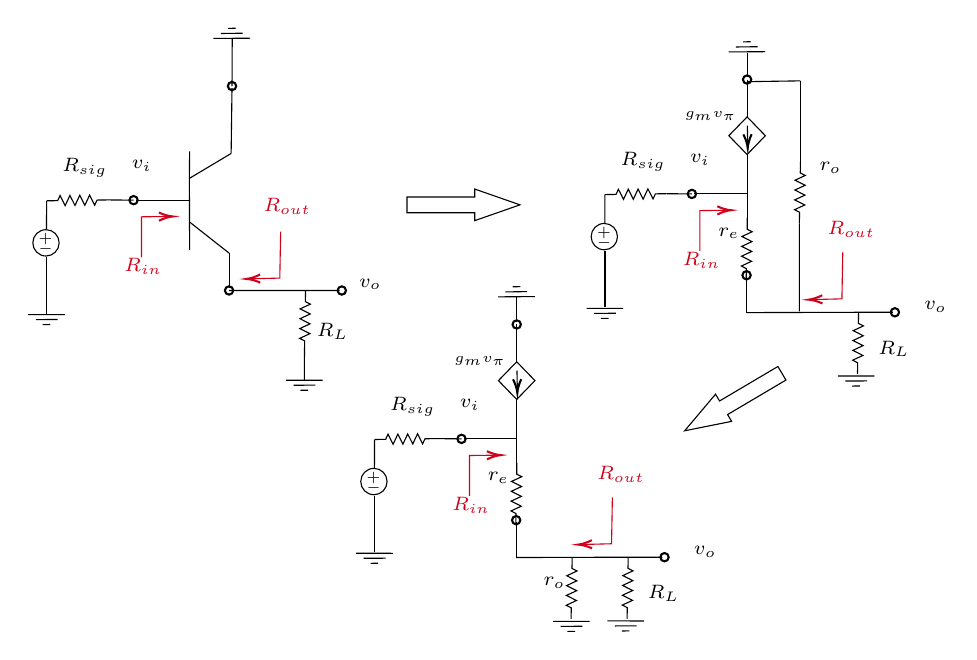
\begin{tikzpicture}[x=0.75pt,y=0.75pt,yscale=-1,xscale=1]
%uncomment if require: \path (0,300); %set diagram left start at 0, and has height of 300

%Straight Lines [id:da4133500324477516] 
\draw    (83.94,67.64) -- (83.82,80.65) -- (83.86,91.14) -- (83.89,101.64) -- (83.94,115.14) ;
%Straight Lines [id:da7830670584441963] 
\draw    (83.82,80.65) -- (103.94,68.64) ;
%Straight Lines [id:da30721918777675417] 
\draw    (83.89,101.64) -- (102.94,116.64) ;
%Straight Lines [id:da9997255942735996] 
\draw    (57.95,91.14) -- (83.86,91.14) ;
\draw [shift={(56.94,91.14)}, rotate = 359.99] [color={rgb, 255:red, 0; green, 0; blue, 0 }  ][line width=0.75]      (0, 0) circle [x radius= 2.01, y radius= 2.01]   ;
%Straight Lines [id:da43133315122711613] 
\draw    (103.94,68.64) -- (104.36,37.17) ;
\draw [shift={(104.37,36.16)}, rotate = 270.77] [color={rgb, 255:red, 0; green, 0; blue, 0 }  ][line width=0.75]      (0, 0) circle [x radius= 2.01, y radius= 2.01]   ;
%Straight Lines [id:da8942046760449994] 
\draw    (102.94,116.64) -- (102.94,133.63) ;
\draw [shift={(102.94,134.64)}, rotate = 90] [color={rgb, 255:red, 0; green, 0; blue, 0 }  ][line width=0.75]      (0, 0) circle [x radius= 2.01, y radius= 2.01]   ;
%Straight Lines [id:da8684535561057921] 
\draw    (102.94,134.64) -- (156.25,134.66) ;
\draw [shift={(157.26,134.66)}, rotate = 0.02] [color={rgb, 255:red, 0; green, 0; blue, 0 }  ][line width=0.75]      (0, 0) circle [x radius= 2.01, y radius= 2.01]   ;
%Straight Lines [id:da45977051079735065] 
\draw    (44.68,91.02) -- (56.94,91.14) ;
%Shape: Circle [id:dp9764375079104787] 
\draw   (8.39,111.7) .. controls (8.39,108.2) and (11.23,105.35) .. (14.74,105.35) .. controls (18.24,105.35) and (21.08,108.2) .. (21.08,111.7) .. controls (21.08,115.2) and (18.24,118.05) .. (14.74,118.05) .. controls (11.23,118.05) and (8.39,115.2) .. (8.39,111.7) -- cycle ;
%Straight Lines [id:da3845153328683255] 
\draw    (15.04,118.45) -- (15.04,145.75) ;
%Straight Lines [id:da46423949264715025] 
\draw    (9.83,148.68) -- (20.32,148.63) ;
%Straight Lines [id:da5793601408315048] 
\draw    (13.13,151.11) -- (16.79,151.06) ;
%Straight Lines [id:da9878557919971883] 
\draw    (6.18,146.25) -- (23.85,146.28) ;

%Straight Lines [id:da5914914926844957] 
\draw    (134.03,180.31) -- (144.52,180.26) ;
%Straight Lines [id:da09483804649922112] 
\draw    (137.33,182.75) -- (140.99,182.7) ;
%Straight Lines [id:da5122315853274279] 
\draw    (130.38,177.88) -- (148.05,177.91) ;

%Straight Lines [id:da2938292496744518] 
\draw    (104.37,36.16) -- (104.47,13) ;
%Straight Lines [id:da20941830503677983] 
\draw    (109.43,10.7) -- (98.95,10.84) ;
%Straight Lines [id:da11007517241569709] 
\draw    (106.12,8.3) -- (102.46,8.38) ;
%Straight Lines [id:da6538432568343695] 
\draw    (113.1,13.1) -- (95.44,13.22) ;

%Right Arrow [id:dp979410899189834] 
\draw   (188.67,89.59) -- (221.32,89.59) -- (221.32,85.79) -- (243.1,93.39) -- (221.32,101) -- (221.32,97.2) -- (188.67,97.2) -- cycle ;
%Shape: Resistor [id:dp43577407497286336] 
\draw   (352.62,99.8) -- (352.53,105.14) -- (354.95,106.37) -- (350.02,108.65) -- (354.87,111.11) -- (349.93,113.4) -- (354.78,115.85) -- (349.85,118.14) -- (354.7,120.6) -- (349.76,122.88) -- (352.19,124.11) -- (352.09,129.45) ;
%Flowchart: Decision [id:dp33499331630798135] 
\draw   (352.53,51.02) -- (361.33,60.08) -- (352.53,69.14) -- (343.73,60.08) -- cycle ;
%Straight Lines [id:da29171091451254105] 
\draw    (352.66,55.23) -- (352.81,63.98) ;
\draw [shift={(352.84,65.98)}, rotate = 269.03] [color={rgb, 255:red, 0; green, 0; blue, 0 }  ][line width=0.75]    (6.56,-1.97) .. controls (4.17,-0.84) and (1.99,-0.18) .. (0,0) .. controls (1.99,0.18) and (4.17,0.84) .. (6.56,1.97)   ;
%Shape: Resistor [id:dp5073701885339131] 
\draw   (15.04,91.45) -- (20.37,91.37) -- (21.52,88.9) -- (23.97,93.76) -- (26.27,88.84) -- (28.71,93.69) -- (31.01,88.77) -- (33.45,93.62) -- (35.75,88.7) -- (38.2,93.56) -- (39.35,91.09) -- (44.68,91.02) ;
%Shape: Resistor [id:dp8922314605853572] 
\draw   (139.8,134.67) -- (139.7,140) -- (142.13,141.23) -- (137.2,143.51) -- (142.04,145.97) -- (137.11,148.26) -- (141.96,150.72) -- (137.03,153) -- (141.88,155.46) -- (136.94,157.74) -- (139.37,158.97) -- (139.27,164.31) ;
%Straight Lines [id:da20174931264036466] 
\draw [color={rgb, 255:red, 208; green, 2; blue, 27 }  ,draw opacity=1 ]   (60.76,118.66) -- (60.76,99.16) -- (73.73,99) ;
\draw [shift={(75.73,98.98)}, rotate = 179.28] [color={rgb, 255:red, 208; green, 2; blue, 27 }  ,draw opacity=1 ][line width=0.75]    (6.56,-1.97) .. controls (4.17,-0.84) and (1.99,-0.18) .. (0,0) .. controls (1.99,0.18) and (4.17,0.84) .. (6.56,1.97)   ;
%Straight Lines [id:da06096463918473072] 
\draw [color={rgb, 255:red, 208; green, 2; blue, 27 }  ,draw opacity=1 ]   (127.79,106.28) -- (127.39,128.68) -- (113.39,129.03) ;
\draw [shift={(111.39,129.08)}, rotate = 358.57] [color={rgb, 255:red, 208; green, 2; blue, 27 }  ,draw opacity=1 ][line width=0.75]    (6.56,-1.97) .. controls (4.17,-0.84) and (1.99,-0.18) .. (0,0) .. controls (1.99,0.18) and (4.17,0.84) .. (6.56,1.97)   ;
%Straight Lines [id:da47582021553536313] 
\draw    (15.04,91.45) -- (14.98,105.08) ;
%Straight Lines [id:da11149077541069974] 
\draw    (139.27,164.31) -- (139.22,177.95) ;
%Straight Lines [id:da656463587264936] 
\draw    (352.53,87.14) -- (352.53,105.14) ;
%Straight Lines [id:da6868937585095206] 
\draw    (352.53,69.14) -- (352.53,87.14) ;
%Straight Lines [id:da21303891052152724] 
\draw    (352.53,33.02) -- (352.53,51.02) ;
%Shape: Resistor [id:dp3835054351957381] 
\draw   (378.24,72.66) -- (378.15,78) -- (380.57,79.23) -- (375.64,81.51) -- (380.49,83.97) -- (375.55,86.26) -- (380.4,88.72) -- (375.47,91) -- (380.32,93.46) -- (375.39,95.74) -- (377.81,96.97) -- (377.71,102.31) ;
%Straight Lines [id:da3545075118783987] 
\draw    (422.73,145.16) -- (406.24,145.16) -- (352.27,145.31) ;
\draw [shift={(423.74,145.16)}, rotate = 180] [color={rgb, 255:red, 0; green, 0; blue, 0 }  ][line width=0.75]      (0, 0) circle [x radius= 2.01, y radius= 2.01]   ;
%Straight Lines [id:da766555053311894] 
\draw    (378.24,33.66) -- (378.24,72.66) ;
%Straight Lines [id:da6700116222154002] 
\draw    (399.86,178.28) -- (410.35,178.23) ;
%Straight Lines [id:da8274222197981748] 
\draw    (403.16,180.71) -- (406.82,180.66) ;
%Straight Lines [id:da2892354184876509] 
\draw    (396.22,175.85) -- (413.88,175.88) ;

%Straight Lines [id:da7462409824382801] 
\draw [color={rgb, 255:red, 208; green, 2; blue, 27 }  ,draw opacity=1 ]   (398.62,116.28) -- (398.22,138.68) -- (384.22,139.03) ;
\draw [shift={(382.22,139.08)}, rotate = 358.57] [color={rgb, 255:red, 208; green, 2; blue, 27 }  ,draw opacity=1 ][line width=0.75]    (6.56,-1.97) .. controls (4.17,-0.84) and (1.99,-0.18) .. (0,0) .. controls (1.99,0.18) and (4.17,0.84) .. (6.56,1.97)   ;
%Straight Lines [id:da8652681052903215] 
\draw    (352.53,32.01) -- (352.53,20.02) ;
\draw [shift={(352.53,33.02)}, rotate = 270] [color={rgb, 255:red, 0; green, 0; blue, 0 }  ][line width=0.75]      (0, 0) circle [x radius= 2.01, y radius= 2.01]   ;
%Straight Lines [id:da3379422722161718] 
\draw    (357.6,17.2) -- (347.11,17.34) ;
%Straight Lines [id:da768322576060915] 
\draw    (354.28,14.8) -- (350.62,14.88) ;
%Straight Lines [id:da133893825661608] 
\draw    (361.27,19.6) -- (343.6,19.72) ;

%Straight Lines [id:da28112724680041834] 
\draw    (352.27,128.32) -- (352.27,145.31) ;
\draw [shift={(352.27,127.31)}, rotate = 90] [color={rgb, 255:red, 0; green, 0; blue, 0 }  ][line width=0.75]      (0, 0) circle [x radius= 2.01, y radius= 2.01]   ;
%Straight Lines [id:da9627475615385244] 
\draw    (326.95,88.14) -- (352.86,88.14) ;
\draw [shift={(325.94,88.14)}, rotate = 359.99] [color={rgb, 255:red, 0; green, 0; blue, 0 }  ][line width=0.75]      (0, 0) circle [x radius= 2.01, y radius= 2.01]   ;
%Straight Lines [id:da6186834699763751] 
\draw    (313.68,88.02) -- (325.94,88.14) ;
%Shape: Circle [id:dp5181398690438553] 
\draw   (277.39,108.7) .. controls (277.39,105.2) and (280.23,102.35) .. (283.74,102.35) .. controls (287.24,102.35) and (290.08,105.2) .. (290.08,108.7) .. controls (290.08,112.2) and (287.24,115.05) .. (283.74,115.05) .. controls (280.23,115.05) and (277.39,112.2) .. (277.39,108.7) -- cycle ;
%Straight Lines [id:da04657431463635331] 
\draw    (284.04,115.45) -- (284.04,142.75) ;
%Straight Lines [id:da8142161183769505] 
\draw    (278.83,145.68) -- (289.32,145.63) ;
%Straight Lines [id:da877292710926374] 
\draw    (282.13,148.11) -- (285.79,148.06) ;
%Straight Lines [id:da44875549029711104] 
\draw    (275.18,143.25) -- (292.85,143.28) ;

%Shape: Resistor [id:dp12916529069775295] 
\draw   (284.04,88.45) -- (289.37,88.37) -- (290.52,85.9) -- (292.97,90.76) -- (295.27,85.84) -- (297.71,90.69) -- (300.01,85.77) -- (302.45,90.62) -- (304.75,85.7) -- (307.2,90.56) -- (308.35,88.09) -- (313.68,88.02) ;
%Straight Lines [id:da38379183322404853] 
\draw [color={rgb, 255:red, 208; green, 2; blue, 27 }  ,draw opacity=1 ]   (329.76,115.66) -- (329.76,96.16) -- (342.73,96) ;
\draw [shift={(344.73,95.98)}, rotate = 179.28] [color={rgb, 255:red, 208; green, 2; blue, 27 }  ,draw opacity=1 ][line width=0.75]    (6.56,-1.97) .. controls (4.17,-0.84) and (1.99,-0.18) .. (0,0) .. controls (1.99,0.18) and (4.17,0.84) .. (6.56,1.97)   ;
%Straight Lines [id:da30040427243759915] 
\draw    (284.04,88.45) -- (283.98,102.08) ;
%Straight Lines [id:da8085278155959004] 
\draw    (352.54,34.05) -- (378.24,33.66) ;
%Straight Lines [id:da5464353478241558] 
\draw    (377.71,102.31) -- (377.74,144.66) ;
%Shape: Resistor [id:dp09379724547967105] 
\draw   (406.24,145.16) -- (406.15,150.5) -- (408.57,151.73) -- (403.64,154.01) -- (408.49,156.47) -- (403.55,158.76) -- (408.4,161.22) -- (403.47,163.5) -- (408.32,165.96) -- (403.39,168.24) -- (405.81,169.47) -- (405.71,174.81) ;
%Shape: Resistor [id:dp21604146155227455] 
\draw   (241.62,217.8) -- (241.53,223.14) -- (243.95,224.37) -- (239.02,226.65) -- (243.87,229.11) -- (238.93,231.4) -- (243.78,233.85) -- (238.85,236.14) -- (243.7,238.6) -- (238.76,240.88) -- (241.19,242.11) -- (241.09,247.45) ;
%Flowchart: Decision [id:dp387299846054486] 
\draw   (241.53,169.02) -- (250.33,178.08) -- (241.53,187.14) -- (232.73,178.08) -- cycle ;
%Straight Lines [id:da23960128480515996] 
\draw    (241.66,173.23) -- (241.81,181.98) ;
\draw [shift={(241.84,183.98)}, rotate = 269.03] [color={rgb, 255:red, 0; green, 0; blue, 0 }  ][line width=0.75]    (6.56,-1.97) .. controls (4.17,-0.84) and (1.99,-0.18) .. (0,0) .. controls (1.99,0.18) and (4.17,0.84) .. (6.56,1.97)   ;
%Straight Lines [id:da9930768193409091] 
\draw    (241.53,205.14) -- (241.53,223.14) ;
%Straight Lines [id:da0046373043587679685] 
\draw    (241.53,187.14) -- (241.53,205.14) ;
%Straight Lines [id:da13587219598838973] 
\draw    (241.53,151.02) -- (241.53,169.02) ;
%Shape: Resistor [id:dp6501423052665937] 
\draw   (268.26,263.24) -- (268.16,268.57) -- (270.59,269.8) -- (265.65,272.09) -- (270.5,274.55) -- (265.57,276.83) -- (270.42,279.29) -- (265.48,281.57) -- (270.33,284.03) -- (265.4,286.32) -- (267.82,287.55) -- (267.73,292.88) ;
%Straight Lines [id:da35409674511600076] 
\draw    (311.73,263.16) -- (295.24,263.16) -- (241.27,263.31) ;
\draw [shift={(312.74,263.16)}, rotate = 180] [color={rgb, 255:red, 0; green, 0; blue, 0 }  ][line width=0.75]      (0, 0) circle [x radius= 2.01, y radius= 2.01]   ;
%Straight Lines [id:da8492371322998509] 
\draw    (288.86,296.28) -- (299.35,296.23) ;
%Straight Lines [id:da21425376588826528] 
\draw    (292.16,298.71) -- (295.82,298.66) ;
%Straight Lines [id:da7102945316890503] 
\draw    (285.22,293.85) -- (302.88,293.88) ;

%Straight Lines [id:da29941637686078526] 
\draw [color={rgb, 255:red, 208; green, 2; blue, 27 }  ,draw opacity=1 ]   (287.62,234.28) -- (287.22,256.68) -- (273.22,257.03) ;
\draw [shift={(271.22,257.08)}, rotate = 358.57] [color={rgb, 255:red, 208; green, 2; blue, 27 }  ,draw opacity=1 ][line width=0.75]    (6.56,-1.97) .. controls (4.17,-0.84) and (1.99,-0.18) .. (0,0) .. controls (1.99,0.18) and (4.17,0.84) .. (6.56,1.97)   ;
%Straight Lines [id:da1986736806718049] 
\draw    (241.53,150.01) -- (241.53,138.02) ;
\draw [shift={(241.53,151.02)}, rotate = 270] [color={rgb, 255:red, 0; green, 0; blue, 0 }  ][line width=0.75]      (0, 0) circle [x radius= 2.01, y radius= 2.01]   ;
%Straight Lines [id:da4361751131395202] 
\draw    (246.6,135.2) -- (236.11,135.34) ;
%Straight Lines [id:da325670718409548] 
\draw    (243.28,132.8) -- (239.62,132.88) ;
%Straight Lines [id:da5880640652658853] 
\draw    (250.27,137.6) -- (232.6,137.72) ;

%Straight Lines [id:da4565706988043702] 
\draw    (241.27,246.32) -- (241.27,263.31) ;
\draw [shift={(241.27,245.31)}, rotate = 90] [color={rgb, 255:red, 0; green, 0; blue, 0 }  ][line width=0.75]      (0, 0) circle [x radius= 2.01, y radius= 2.01]   ;
%Straight Lines [id:da9342338138030444] 
\draw    (215.95,206.14) -- (241.86,206.14) ;
\draw [shift={(214.94,206.14)}, rotate = 359.99] [color={rgb, 255:red, 0; green, 0; blue, 0 }  ][line width=0.75]      (0, 0) circle [x radius= 2.01, y radius= 2.01]   ;
%Straight Lines [id:da9547449697354166] 
\draw    (202.68,206.02) -- (214.94,206.14) ;
%Shape: Circle [id:dp8968296253605997] 
\draw   (166.39,226.7) .. controls (166.39,223.2) and (169.23,220.35) .. (172.74,220.35) .. controls (176.24,220.35) and (179.08,223.2) .. (179.08,226.7) .. controls (179.08,230.2) and (176.24,233.05) .. (172.74,233.05) .. controls (169.23,233.05) and (166.39,230.2) .. (166.39,226.7) -- cycle ;
%Straight Lines [id:da8955610240005476] 
\draw    (173.04,233.45) -- (173.04,260.75) ;
%Straight Lines [id:da5182675065936346] 
\draw    (167.83,263.68) -- (178.32,263.63) ;
%Straight Lines [id:da4732213137601031] 
\draw    (171.13,266.11) -- (174.79,266.06) ;
%Straight Lines [id:da6195072134501105] 
\draw    (164.18,261.25) -- (181.85,261.28) ;

%Shape: Resistor [id:dp3029249545726985] 
\draw   (173.04,206.45) -- (178.37,206.37) -- (179.52,203.9) -- (181.97,208.76) -- (184.27,203.84) -- (186.71,208.69) -- (189.01,203.77) -- (191.45,208.62) -- (193.75,203.7) -- (196.2,208.56) -- (197.35,206.09) -- (202.68,206.02) ;
%Straight Lines [id:da8945343820671074] 
\draw [color={rgb, 255:red, 208; green, 2; blue, 27 }  ,draw opacity=1 ]   (218.76,233.66) -- (218.76,214.16) -- (231.73,214) ;
\draw [shift={(233.73,213.98)}, rotate = 179.28] [color={rgb, 255:red, 208; green, 2; blue, 27 }  ,draw opacity=1 ][line width=0.75]    (6.56,-1.97) .. controls (4.17,-0.84) and (1.99,-0.18) .. (0,0) .. controls (1.99,0.18) and (4.17,0.84) .. (6.56,1.97)   ;
%Straight Lines [id:da08295517977573585] 
\draw    (173.04,206.45) -- (172.98,220.08) ;
%Shape: Resistor [id:dp3690950789893612] 
\draw   (295.24,263.16) -- (295.15,268.5) -- (297.57,269.73) -- (292.64,272.01) -- (297.49,274.47) -- (292.55,276.76) -- (297.4,279.22) -- (292.47,281.5) -- (297.32,283.96) -- (292.39,286.24) -- (294.81,287.47) -- (294.71,292.81) ;
%Straight Lines [id:da4390238476139843] 
\draw    (262.66,296.48) -- (273.15,296.43) ;
%Straight Lines [id:da7782276316254176] 
\draw    (265.96,298.91) -- (269.62,298.86) ;
%Straight Lines [id:da4990687255417269] 
\draw    (259.02,294.05) -- (276.68,294.08) ;

%Right Arrow [id:dp8993377958648644] 
\draw   (371.24,177.81) -- (343.13,194.44) -- (345.07,197.71) -- (322.46,202.25) -- (337.33,184.62) -- (339.26,187.89) -- (367.37,171.27) -- cycle ;

% Text Node
\draw (9.86,105.92) node [anchor=north west][inner sep=0.75pt]  [font=\tiny]  {$+$};
% Text Node
\draw (9.71,110.63) node [anchor=north west][inner sep=0.75pt]  [font=\tiny]  {$-$};
% Text Node
\draw (54.83,70.73) node [anchor=north west][inner sep=0.75pt]  [font=\scriptsize]  {$v_{i}$};
% Text Node
\draw (164.33,127.73) node [anchor=north west][inner sep=0.75pt]  [font=\scriptsize]  {$v_{o}$};
% Text Node
\draw (337.4,103.13) node [anchor=north west][inner sep=0.75pt]  [font=\scriptsize]  {$r_{e}$};
% Text Node
\draw (321.23,47.38) node [anchor=north west][inner sep=0.75pt]  [font=\tiny]  {$g_{m} v_{\pi }$};
% Text Node
\draw (21.32,69.86) node [anchor=north west][inner sep=0.75pt]  [font=\scriptsize]  {$R_{sig}$};
% Text Node
\draw (144.04,149.37) node [anchor=north west][inner sep=0.75pt]  [font=\scriptsize]  {$R_{L}$};
% Text Node
\draw (51.27,117.92) node [anchor=north west][inner sep=0.75pt]  [font=\scriptsize,color={rgb, 255:red, 208; green, 2; blue, 27 }  ,opacity=1 ]  {$R_{in}$};
% Text Node
\draw (118.27,89.12) node [anchor=north west][inner sep=0.75pt]  [font=\scriptsize,color={rgb, 255:red, 208; green, 2; blue, 27 }  ,opacity=1 ]  {$R_{out}$};
% Text Node
\draw (436.67,138.73) node [anchor=north west][inner sep=0.75pt]  [font=\scriptsize]  {$v_{o}$};
% Text Node
\draw (414.46,157.63) node [anchor=north west][inner sep=0.75pt]  [font=\scriptsize]  {$R_{L}$};
% Text Node
\draw (390.1,100.12) node [anchor=north west][inner sep=0.75pt]  [font=\scriptsize,color={rgb, 255:red, 208; green, 2; blue, 27 }  ,opacity=1 ]  {$R_{out}$};
% Text Node
\draw (278.86,102.92) node [anchor=north west][inner sep=0.75pt]  [font=\tiny]  {$+$};
% Text Node
\draw (278.71,107.63) node [anchor=north west][inner sep=0.75pt]  [font=\tiny]  {$-$};
% Text Node
\draw (323.83,67.73) node [anchor=north west][inner sep=0.75pt]  [font=\scriptsize]  {$v_{i}$};
% Text Node
\draw (290.32,66.86) node [anchor=north west][inner sep=0.75pt]  [font=\scriptsize]  {$R_{sig}$};
% Text Node
\draw (320.27,114.92) node [anchor=north west][inner sep=0.75pt]  [font=\scriptsize,color={rgb, 255:red, 208; green, 2; blue, 27 }  ,opacity=1 ]  {$R_{in}$};
% Text Node
\draw (386.2,71.46) node [anchor=north west][inner sep=0.75pt]  [font=\scriptsize]  {$r_{o}$};
% Text Node
\draw (226.4,221.13) node [anchor=north west][inner sep=0.75pt]  [font=\scriptsize]  {$r_{e}$};
% Text Node
\draw (210.23,165.38) node [anchor=north west][inner sep=0.75pt]  [font=\tiny]  {$g_{m} v_{\pi }$};
% Text Node
\draw (325.67,256.73) node [anchor=north west][inner sep=0.75pt]  [font=\scriptsize]  {$v_{o}$};
% Text Node
\draw (303.46,275.63) node [anchor=north west][inner sep=0.75pt]  [font=\scriptsize]  {$R_{L}$};
% Text Node
\draw (279.1,218.12) node [anchor=north west][inner sep=0.75pt]  [font=\scriptsize,color={rgb, 255:red, 208; green, 2; blue, 27 }  ,opacity=1 ]  {$R_{out}$};
% Text Node
\draw (167.86,220.92) node [anchor=north west][inner sep=0.75pt]  [font=\tiny]  {$+$};
% Text Node
\draw (167.71,225.63) node [anchor=north west][inner sep=0.75pt]  [font=\tiny]  {$-$};
% Text Node
\draw (212.83,185.73) node [anchor=north west][inner sep=0.75pt]  [font=\scriptsize]  {$v_{i}$};
% Text Node
\draw (179.32,184.86) node [anchor=north west][inner sep=0.75pt]  [font=\scriptsize]  {$R_{sig}$};
% Text Node
\draw (209.27,232.92) node [anchor=north west][inner sep=0.75pt]  [font=\scriptsize,color={rgb, 255:red, 208; green, 2; blue, 27 }  ,opacity=1 ]  {$R_{in}$};
% Text Node
\draw (253.2,271.46) node [anchor=north west][inner sep=0.75pt]  [font=\scriptsize]  {$r_{o}$};
\end{tikzpicture}
\end{center}
計算$A_v \equiv \frac{v_o}{v_i}$
\begin{align*}
	\because v_o &= v_i \frac{r_o || R_L}{r_e + (r_o || R_L)} \\
	\therefore A_v &= \frac{r_o || R_L}{r_e + (r_o || R_L)} \\
	\text since \quad r_e &\ll r_o || R_L \\
	\Rightarrow A_v &\approx 1
\end{align*}

計算 $G_v \equiv \frac{v_{\text{sig}}}{v_i}$
\begin{align*}
	v_i &= v_{\text{sig}} \frac{R_\text{in}}{R_{\text{in}} + R_{\text{sig}}} \\
	R_{\text{in}} &= \frac{v_i}{(1/(1+ \beta))i_e}
								= \frac{v_i}{(1/(1+\beta)) \frac{v_i}{r_e + (r_o || R_L)}}\\
								&= (1+\beta)(r_e + r_o || R_L)
\end{align*}
\textbf{Summary of CE Amp. (It can be buffer Amp.)} \\
\begin{center}
	\begin{minipage}{0.6\textwidth}
		\begin{enumerate}[label=\arabic*.]
		  \item $R_{\text{in}} = (1+\beta)(r_e + r_o || R_L), R_{\text{in}}$ very high
			\item $R_{\text{out}} = \frac{R_{\text{sig}}}{1+\beta}+r_e$ very low
			\item $A_v \approx 1$
		\end{enumerate}
	\end{minipage}
\end{center}


\end{document}
